% !TEX program = lualatex
\documentclass[10pt, leqno]{ltjsarticle}
% \documentclass[10pt]{ltjsarticle} % 日本語をそのまま扱えるクラス
% \usepackage[margin=28mm]{geometry}
\usepackage{amsmath,amssymb,mathtools}
\usepackage{amsthm}
\usepackage{tikz}
\usetikzlibrary{arrows.meta,positioning,calc}

\usepackage[
  top=15mm,     % 上余白
  bottom=15mm,  % 下余白
  left=10mm,    % 左余白
  right=10mm,    % 右余白
  landscape,
  margin=10mm
]{geometry}
% \usepackage[landscape,margin=20mm]{geometry} % 余白はお好みで
\usepackage{paracol}
\columnratio{0.5,0.5}             % 左右を 1:1 に
\setlength{\columnseprule}{0.4pt} % 真ん中の縦線

\usepackage{titlesec}
\titleformat{\paragraph}
  {\normalfont\bfseries}
  {}      % ← 番号を空に
  {0pt}
  {}

% ---- 記号・マクロ ----
\newcommand{\xto}{\mathrel{\xrightarrow{}}}
\newcommand{\into}{\hookrightarrow}
\newcommand{\epi}{\twoheadrightarrow}
\newcommand{\pto}{\rightrightarrows}
\newcommand{\cls}[1]{\bigl(#1\bigr)}
\newcommand{\redjoin}{\wedge}
\newcommand{\shrink}{\phi}
\newcommand{\Ex}{E}        % suspension functor E
\newcommand{\Ox}{\Omega}   % loop functor Omega
\newcommand{\id}{\mathrm{id}}
% --- Toda bracket helpers ---
\newcommand{\toda}[1]{\{\,#1\,\}}              % {a,b,c}
\newcommand{\todai}[2][]{\{\,#2\,\}_{#1}}      % {a,b,c}_i   (#1 は添字, 空なら無し) 
\newcommand{\gen}[1]{\{\,#1\,\}}       % ⟨generator⟩ 表記を { } で統一
\newcommand{\Ker}{\operatorname{Ker}}
\newcommand{\im}{\operatorname{Im}}
\newcommand{\hs}[2]{\bigl[#1,#2\bigr]}   % 一般のホモトピー集合
\newcommand{\pis}[2]{\pi_{#1}(#2)}       % 左が球面のときのホモトピー群
\newcommand{\pit}[2]{\pi_{#1}^{#2}}
\newcommand{\ext}[1]{\overline{#1}}     % extension
\newcommand{\coext}[1]{\widetilde{#1}}  % coextension
\newcommand{\z}{\mathbb{Z}}

% ---- theorem-like environments ----
\numberwithin{equation}{section}
\theoremstyle{plain}
\newtheorem{theorem}{Theorem}[section]
\newtheorem{lemma}[theorem]{Lemma}
\newtheorem{proposition}[theorem]{Proposition}
\newtheorem{corollary}[theorem]{Corollary}
\theoremstyle{definition}
\newtheorem{definition}[theorem]{Definition}
\newtheorem{example}[theorem]{Example}
\newtheorem{notation}[theorem]{Notation}
\newtheorem{assumption}[theorem]{Assumption}
\theoremstyle{remark}
\newtheorem{remark}[]{Remark}

% \title{PART 1 \quad CHAPTER I\\[2mm] General Composition and Secondary Composition}
\author{}
\date{}

\begin{document}

\setcounter{section}{5}
\section{Some Elements Given By Secondary Compositions}

\begin{paracol}{2}

\paragraph{i). The Elements \(\varepsilon_n\).}

Toda bracket \(\todai[1]{\eta_3,\ E\nu',\ \nu_7}\) を考える. \\
(1.13) の条件, \(\eta_3\circ E\nu'= \nu'\circ \nu_6 =0\) 
は, Lem5.7 と Prop5.11 から満たされる. \\
したがって, この Toda bracket は定義され, 次の部分群の coset である：
\[
\eta_3\circ E\,\pi_{10}(S^3)\;+\;\pi_{8}(S^3)\circ \nu_8
\ =\ \eta_3\circ E\,\pi^{3}_{10}\;+\;\pi^{3}_{8}\circ \nu_8 \quad\text{by (4.7)}
\]
\[
=\ \gen{\ \nu'\circ \eta_6^{\,2}\circ \nu_8\ }\ =\ 0
\quad\text{by Prop5.15, 5.9} \ .
\]
ゆえに, この Toda bracket は単一元から成り, その元について次のように定める.
\[
\varepsilon_3\ :=\ \todai[1]{\eta_3,\ E\nu',\ \nu_7}\ \in \pi_{11}(S^3),
\]
\[
\varepsilon_n:=E^{\,n-3}\varepsilon_3\quad (n\ge3),\qquad
\varepsilon:=E^{\infty}\varepsilon_3.
\]

\begin{lemma}\label{lem:6.1}
% \noindent
% \textbf{Lem6.1.}\
\(H(\varepsilon_3)=\nu_5^{\,2}\) , 
\(2\varepsilon_n=2\varepsilon=0\ ,(n\ge3)\). 
\end{lemma}

\noindent
\textbf{Proof.}\
Lem5.7 より, \(\eta_2\circ \nu'=\pm\,\Delta(\nu_5) .\)
Prop2.6 から,
\[
\nu_5^{\,2}\ =\ \pm\,\nu_5\circ \nu_8\ \in\ \Delta^{-1}(\eta_2\circ \nu')\circ \nu_8
\ =\ H\todai[1]{\eta_3,\ E\nu',\ \nu_7}.
\]
\(\todai[1]{\eta_3,E\nu',\nu_7} = \varepsilon_3\) なので,
\(H(\varepsilon_3)=\nu_5^{\,2}\).
次に,
\[
\begin{align*}
2\varepsilon_3
&= 2\iota_3\circ \varepsilon_3 \in 2\iota_3\circ \todai[1]{\eta_3,E\nu',\nu_7}
&& \text{by Lem4.5}\\
&= \toda{2\iota_3,\eta_3,E\nu'}\circ \nu_8\\
&\subset \pis{8}{S^3}\circ\nu_8 = \pit{8}{3}\circ\nu_8 
&& \text{(4.7)}\\
&= \gen{\ \nu'\circ \eta_6^{2}\circ \nu_8\ }
&& \text{by Prop5.9}\\
&= 0 
&& \text{(5.9).}
\end{align*}
\]
これから, 明らかに \(2\varepsilon_n=2\varepsilon=0\) である. 
\qed
% ==== CHAPTER VI p.52 ====
\begin{equation}\label{eq:6.1}
% \noindent
%(6.1).\ 
\text{次の Toda bracket は } \varepsilon_n \text{ を含んでいる. }\quad
\end{equation}

\noindent
\(n\ge4,\ 0\le t\le n-2\) に対して, 
\[
\todai[t]{\eta_n,\ 2\nu_{n+1},\ \nu_{n+4}},
\]
\(n\ge5,\ 0\le t\le n-5\) に対して, 
\[
\todai[t]{\eta_n, \nu_{n+1}, 2\nu_{n+4}},\
\todai[t]{\eta_n, 2\iota_{n+1}, \nu_{n+1}^2},\
\todai[t]{\eta_n,\ \nu_{n+1}^{2},\ \iota_{n+7}} .
\]

\switchcolumn

\noindent
$n\ge 0$ を整数とし, 
$\alpha\in[\Ex^n Y, Z]$, $\beta\in[X, Y]$, $\gamma\in[W, X]$ に対して,\\
\textbf{(1.13).}\
\(\alpha\circ \Ex^n\beta=0,\ \beta\circ \gamma=0\).

\noindent
\textbf{Lem5.7.}\
\(\alpha\in\pi_i(S^3)\) に対して,
\(E^2\alpha\in2\iota_5\circ\pi_{i+2}(S^5)\) ならば, 
\(E(\eta_2\circ\alpha)=0\) である. \\
特に, \(E(\eta_2\circ\nu')=0, \ \Delta(\nu_5)=\pm(\eta_2\circ\nu')\) である. 

\noindent
\textbf{Prop5.11.}\
\(\pi^{2}_{8}=\mathbb Z_2\gen{\eta_{2}\circ\nu'\circ\eta_6^2},\)\quad 
\(\pi^{3}_{9}=0,\)\quad \(\pi^{4}_{10}=\mathbb Z_8\gen{\nu_{4}^2},\) \\
\(\pi^{n}_{n+6}=\mathbb Z_2\gen{\nu_n^2}\ (n\ge5),\) \
\((G_{6};2)=\mathbb Z_2\gen{\nu^2}.\)

\noindent
\textbf{(4.7).}\
\(n\ge1, \ \alpha\in\pis{k+n}{S^m; 2},\ \gamma\in\pis{i}{S^j; 2}
    \ \text{のとき, }\)\\
\(\alpha\circ E^n\pis{j}{S^k} = \alpha\circ E^n \pit{j}{k}
  \subset \pit{j+n}{m},
  \ \pis{j}{S^k}\circ\gamma = \pit{j}{k}\circ\gamma \subset\pit{i}{k}\ . \)\\
\(\text{さらに, }\ \alpha\circ E^n\beta=0,\ \beta\circ\gamma = 0 \ \text{のとき, }\)\\
\(\todai[n]{\alpha, E^n\beta, E^n\gamma}\ \text{は,}\
  \alpha\circ E^n\pit{i+1}{k} + \pit{j+n+1}{m}\circ E^{n+1}\gamma\
  \text{の coset で, }\pit{i+n+1}{m} \ \text{の部分集合である. }\)

\noindent
\textbf{Prop5.15.}\
\(\pi_9^2=\pi_{10}^3=\pi_{11}^4=0,\) \\
\(\pi^{5}_{12}=\mathbb Z_2\gen{\sigma'''},\) \
\(\pi^{6}_{13}=\mathbb Z_4\gen{\sigma''},\) \
\(\pi^{7}_{14}=\mathbb Z_8\gen{\sigma'},\) \
\(\pi^{8}_{15}=\mathbb Z\gen{\sigma_8}\oplus\mathbb Z\gen{E\sigma'},\) \\
\(\pi^{n}_{n+7}=\mathbb Z_{16}\gen{\sigma_n}\ (n\ge9),\) \
\((G_{7};2)=\mathbb Z_{16}\gen{\sigma}.\)

\noindent
\textbf{Prop5.9.}\
\(\pi^{2}_{7}=\mathbb Z_2\gen{\eta_{2}\circ\nu'\circ\eta_6},\) \quad
\(\pi^{3}_{8}=\mathbb Z_2\gen{\nu'\circ\eta_6^2},\) \quad
\(\pi^{4}_{9}=\mathbb Z_2\gen{\nu_{4}\circ\eta_7^2}\oplus \mathbb Z_2\gen{E\nu'\circ\eta_7^2},\) \\
\(\pi^{5}_{10}=\mathbb Z_2\gen{\nu_{5}\circ\eta_8^2},\) \quad
\(\pi^{6}_{11}=\mathbb Z_2\gen{\Delta(\iota_{13})},\) \quad
\(\pi^{n}_{n+5}=0\ (n\ge7),\) \
\((G_{5};2)=0.\)

\noindent
\textbf{Lem5.7.}\
\(\alpha\in\pi_i(S^3)\) に対して,
\(E^2\alpha\in2\iota_5\circ\pi_{i+2}(S^5)\) ならば, 
\(E(\eta_2\circ\alpha)=0\) である. \\
特に, \(E(\eta_2\circ\nu')=0, \ \Delta(\nu_5)=\pm(\eta_2\circ\nu')\) である. 

\noindent
\textbf{Prop2.6.}\
\(H\todai[1]{E\alpha, E\beta, E\gamma} 
= -\Delta^{-1}(\alpha\circ\beta)\circ E^2\gamma.\)

\noindent
\textbf{Lem4.5.}\
\(n=2,4,8\) のとき, 
\(E:\pis{i-1}{S^n-1}\to\pis{i}{S^n}\) は単射.\\ 
\(r\iota_{n-1}\circ\beta = r\beta,\ \beta\in\pis{i-1}{S^{n-1}}\).

\noindent
\textbf{(4.7).}\
\(n\ge1, \ \alpha\in\pis{k+n}{S^m; 2},\ \gamma\in\pis{i}{S^j; 2}
    \ \text{のとき, }\)\\
\(\alpha\circ E^n\pis{j}{S^k} = \alpha\circ E^n \pit{j}{k}
  \subset \pit{j+n}{m},
  \ \pis{j}{S^k}\circ\gamma = \pit{j}{k}\circ\gamma \subset\pit{i}{k}\ . \)\\
\(\text{さらに, }\ \alpha\circ E^n\beta=0,\ \beta\circ\gamma = 0 \ \text{のとき, }\)\\
\(\todai[n]{\alpha, E^n\beta, E^n\gamma}\ \text{は,}\
  \alpha\circ E^n\pit{i+1}{k} + \pit{j+n+1}{m}\circ E^{n+1}\gamma\
  \text{の coset で, }\pit{i+n+1}{m} \ \text{の部分集合である. }\)

\noindent
\textbf{(5.9).}\
\(\eta_3\circ \nu_4= \nu'\circ \eta_6,\
\eta_n\circ \nu_{n+1}=0\ (n\ge5),\
\nu_n\circ \eta_{n+3}=0\ (n\ge6)\)






\end{paracol}

\begin{paracol}{2}

\noindent
\textbf{Proof.}\
Prop1.3 と (1.15) より, 
\(n\ge4,\ 0\le t\le n-2\) に対して, 
\[
\begin{align*}
\varepsilon_n 
&= (-1)^{n-3}E^{\,n-3}\varepsilon_3
\in (-1)^{n-3}E^{\,n-3}\todai[1]{\eta_3,E\nu',\nu_7}\\
&\subset \todai[n-2]{\eta_n,\ 2\nu_{n+1},\ \nu_{n+4}}\\
&\subset \todai[t]{\eta_n,\ 2\nu_{n+1},\ \nu_{n+4}}
\end{align*}
\]

次に, Toda bracket \(\todai[1]{\eta_5,\ 2\nu_6,\ \nu_9}\) を考える. \\
(4.7) より, これは
\(\eta_5\circ E\,\pi^{5}_{12}+\pi^{5}_{10}\circ \nu_{10}\) の coset である. \\
Prop5.15 と Lem5.14 から,
\(\eta_5\circ E\,\pi^{5}_{12}\) は, 
\(\eta_5\circ E\sigma''' = \eta_5\circ 2 E\sigma''\) 
により生成される. \\
(5.14) により,
\(E:\pit{13}{6}\to\pit{14}{7}\) は単射である. \\
\(E(2\iota_6\circ\sigma'' - E\sigma''') 
= 2E\sigma'' - E2\sigma'' = 0\) 
なので, 
\(2\iota_6\circ\sigma'' = E\sigma'''\) である. \\
よって, \(\eta_5\circ E\sigma''' = \eta_5\circ2\iota_6\circ\sigma'' = 0,\
\eta_5\circ E\pit{12}{5} = 0\) である. \\
Prop5.9 と (5.9) により, 
\(\pi^{5}_{10}\circ \nu_{10} = \gen{\nu_5\circ \eta_8^2\circ \nu_{10}} = 0 .\) \\
したがって, \(\todai[1]{\eta_5,2\nu_6,\nu_9}\) は自明部分群の coset で, 
ただ 1 個の元 \(\varepsilon_5\) から成る. \\
Prop1.2 から,
\[
\todai[1]{\eta_5,\ \nu_6,\ 2\nu_9}\subset
\todai[1]{\eta_5,\ 2\nu_6,\ \nu_9},\qquad
\todai[1]{\eta_5,\ 2\iota_6,\ \nu_6^2}\subset
\todai[1]{\eta_5,\ 2\nu_6,\ \nu_9}.
\]
よって,
\(\todai[1]{\eta_5, \nu_6, 2\nu_9}, \ \todai[1]{\eta_5, 2\iota_6, \nu_6^2}\)
は, \(\varepsilon_5\) だけから成る. 
同様に, 
\[
\varepsilon_5\in \todai[1]{\eta_5, \nu_6, 2\nu_9}
\subset \todai[1]{\eta_5, \nu_6^2, 2\iota_{12}} .
\]
以上から, \(n=5\) に対して, (6.1) が成り立つ. \\
\(n\ge6\) の場合についての証明も, この証明の前半と同様である. 
\qedhere
\qed
\begin{equation}\label{eq:6.2}
% \noindent
% (6.2).\ 
\sigma'''\circ \nu_{12}\ \equiv\ \eta_5^{\,2}\circ \varepsilon_7
\mod{4(\nu_5\circ E\sigma')} .
\end{equation}

\noindent
\textbf{Proof.}\
\(\todai[3]{\nu_5,\ 8\iota_8,\ \nu_8^{\,2}}\) は, 
(4.7) より,
\(\nu_5\circ E^3\,\pi^{5}_{12}+\pi^{5}_{9}\circ \nu_9^{\,2}\) の coset である. \\
Prop5.15 と Lem5.14 から,
\[
\nu_5\circ E^3\,\pi^{5}_{12}
=\gen{\nu_5\circ E^{3}\sigma'''}
=\gen{4(\nu_5\circ E\sigma')} .
\]
また, Prop5.8 と (5.9) より, 
\[
\pi^{5}_{9}\circ \nu_9^{\,2} = \gen{\nu_5\circ\eta_8\circ\nu_9^2} = 0 .
\]
ゆえに, \(\todai[3]{\nu_5,8\iota_8,\nu_8^{\,2}}\) は,
\(\gen{4(\nu_5\circ E\sigma')}\) の coset である. \\
Prop1.2 とLem5.13 から,
\[
\sigma'''\circ \nu_{12}\ \in\
\todai[3]{\nu_5,8\iota_8,\nu_8}\circ \nu_{12}
\subset \todai[3]{\nu_5,8\iota_8,\nu_8^{\,2}}.
\]

\switchcolumn

\noindent
\textbf{Prop1.3.}\
\(-E\todai[n]{\alpha, E^n\beta, E^n\gamma}
\subset \todai[n+1]{E\alpha, E^{n+1}\beta, E^{n+1}\gamma}\).

\noindent
\textbf{(1.15).}\
\(\{\alpha,\ \Ex^n\beta,\ \Ex^n\gamma\}_n
\ \subset\
\bigl\{\alpha,\ \Ex^{m}(E^{n-m}\beta),\ E^{m}(E^{n-m}\gamma)\bigr\}_m .\)

\noindent
\textbf{(4.7).}\
\(n\ge1, \ \alpha\in\pis{k+n}{S^m; 2},\ \gamma\in\pis{i}{S^j; 2}
    \ \text{のとき, }\)\\
\(\alpha\circ E^n\pis{j}{S^k} = \alpha\circ E^n \pit{j}{k}
  \subset \pit{j+n}{m},
  \ \pis{j}{S^k}\circ\gamma = \pit{j}{k}\circ\gamma \subset\pit{i}{k}\ . \)\\
\(\text{さらに, }\ \alpha\circ E^n\beta=0,\ \beta\circ\gamma = 0 \ \text{のとき, }\)\\
\(\todai[n]{\alpha, E^n\beta, E^n\gamma}\ \text{は,}\
  \alpha\circ E^n\pit{i+1}{k} + \pit{j+n+1}{m}\circ E^{n+1}\gamma\
  \text{の coset で, }\pit{i+n+1}{m} \ \text{の部分集合である. }\)

\noindent
\textbf{Prop5.15.}\
\(\pi_9^2=\pi_{10}^3=\pi_{11}^4=0,\) \\
\(\pi^{5}_{12}=\mathbb Z_2\gen{\sigma'''},\) \
\(\pi^{6}_{13}=\mathbb Z_4\gen{\sigma''},\) \
\(\pi^{7}_{14}=\mathbb Z_8\gen{\sigma'},\) \
\(\pi^{8}_{15}=\mathbb Z\gen{\sigma_8}\oplus\mathbb Z\gen{E\sigma'},\) \\
\(\pi^{n}_{n+7}=\mathbb Z_{16}\gen{\sigma_n}\ (n\ge9),\) \
\((G_{7};2)=\mathbb Z_{16}\gen{\sigma}.\)

\noindent
\textbf{Lem5.14.}\
\(\sigma_{8}\in\pi^{8}_{15}\ , \ \sigma'\in\pi^{7}_{14}\ , \ \sigma''\in\pi^{6}_{13}\) 
が存在して, 次を満たす. \\
\(H(\sigma_{8})=\iota_{15} \ ,\quad 2E\sigma_{8}=E^{2}\sigma',\)\\
\(H(\sigma')=\eta_{13} \ ,\quad 2\sigma'=E\sigma'',\)\\
\(H(\sigma'')=\eta_{11}^2 \ ,\quad 2\sigma''=E\sigma''' .\)

\noindent
\textbf{(5.14).}\
次の列は完全列である.\\
\(
0\to \pi^{5}_{12}\xrightarrow{E}\pi^{6}_{13}\xrightarrow{H}\pi^{11}_{13}\to0,
\quad
0\to \pi^{6}_{13}\xrightarrow{E}\pi^{7}_{14}\xrightarrow{H}\pi^{13}_{14}\to0 .
\)

\noindent
\textbf{Prop5.9.}\
\(\pi^{2}_{7}=\mathbb Z_2\gen{\eta_{2}\circ\nu'\circ\eta_6},\) \quad
\(\pi^{3}_{8}=\mathbb Z_2\gen{\nu'\circ\eta_6^2},\) \quad
\(\pi^{4}_{9}=\mathbb Z_2\gen{\nu_{4}\circ\eta_7^2}\oplus \mathbb Z_2\gen{E\nu'\circ\eta_7^2},\) \\
\(\pi^{5}_{10}=\mathbb Z_2\gen{\nu_{5}\circ\eta_8^2},\) \quad
\(\pi^{6}_{11}=\mathbb Z_2\gen{\Delta(\iota_{13})},\) \quad
\(\pi^{n}_{n+5}=0\ (n\ge7),\) \
\((G_{5};2)=0.\)

\noindent
\textbf{(5.9).}\
\(\eta_3\circ \nu_4= \nu'\circ \eta_6,\
\eta_n\circ \nu_{n+1}=0\ (n\ge5),\
\nu_n\circ \eta_{n+3}=0\ (n\ge6)\)

\noindent
\textbf{Prop1.2.}\
\textbf{0).}\ $\alpha$, $\beta$, $\gamma$ のうち, いずれかが $0$ なら,
\(
\{\alpha,\ \Ex^n\beta,\ \Ex^n\gamma\}_n\equiv0.
\)\\
\textbf{i).}\ $\alpha\circ \Ex^n\beta=\beta\circ\gamma=0$ のとき,
\(
\{\alpha,\ \Ex^n\beta,\ \Ex^n\gamma\}_n\circ\Ex^{n+1}\delta\ \subset\ \{\alpha,\Ex^n \beta, \Ex^n(\gamma\circ\delta)\}_n.
\)\\
\textbf{ii).}\ $\alpha\circ \Ex^n\beta=\beta\circ\gamma\circ\delta=0$ のとき,
\(
\{\alpha,\ \Ex^n\beta,\ \Ex^n(\gamma\circ\delta)\}_n\ \subset\ \{\alpha,\ \Ex^n(\beta\circ\gamma),\ \Ex^n\delta\}_n .
\)\\
\textbf{iii).}\ $\alpha\circ\Ex^n\beta\circ\Ex^n\gamma=\gamma\circ\delta=0$ なら,
\(
\{\alpha\circ\Ex^n\beta,\ \Ex^n\gamma,\ \Ex^n\delta)\}_n\ \subset\ \{\alpha,\ \Ex^n(\beta\circ\gamma),\ \Ex^n\delta\}_n .
\)\\
\textbf{iv).}\ $\beta\circ\Ex^n\gamma=\gamma\circ\delta=0$ のとき,
\(
\alpha\circ\{\beta,\ \Ex^n\gamma,\ \Ex^n\delta\}_n\ \subset\ \{\alpha\circ\beta,\ \Ex^n\gamma,\ \Ex^n\delta\}_n .
\)

\noindent
\textbf{Lem5.13.}\
\(\todai[t]{\nu_5,8\iota_8,\nu_8},\ (0\leq t\leq3)\) 
は, ただ$1$つの元から成る. \\
この元を \(\sigma'''\) と書くと, 
\(H(\sigma''')=4\nu_9=\eta_9^3\) であり, \\
\(\pi_{12}^5=\mathbb{Z}_2\gen{\sigma'''}\)
である. 







\end{paracol}

\begin{paracol}{2}

\noindent
一方, (6.1) とProp1.2 より,
\[
\begin{align*}
\eta_5^{\,2}\circ \varepsilon_7
&\in \eta_5^2\circ\todai[3]{\eta_7,2\iota_8,\nu_8^{\,2}} \\
&\subset \todai[3]{\eta_5^3, 2\iota_8, \nu_8^2}
= \todai[3]{4\nu_5, 2\iota_8, \nu_8^2}\\
&\subset \todai[3]{\nu_5,8\iota_8,\nu_8^{\,2}} .
\end{align*}
\]
したがって, 
\(\sigma''' \circ\nu_{12}\) と \(\eta_5^2\circ\varepsilon_7\) は, 
\(4(\nu_5\circ E\sigma')\) の同じ coset の元である. \\
以上で, (6.2) が確かめられた. 
\qed


% ==== CHAPTER VI p.53 ====

\paragraph{ii). The elements \(\,\overline{\nu}_n\).}

Toda bracket 
\[
\todai[t]{\nu_6,\ \eta_9,\ \nu_{10}}\qquad(0\le t\le 4)
\]
は, (5.9) の関係式より定義され,  (4.7) より, これは,
\[
\pi^{6}_{11}\circ \nu_{11}+\nu_6\circ E^t\pis{14-t}{S^{9-t}}
\]
の coset である. 
\(\pis{14}{S^9}\) は stable, すなわち, 
\(\pis{14}{S^9} = E\pis{13}{S^8}\)
なので, 
\[
\nu_6\circ E^t\pis{14-t}{S^{9-t}} 
\subset\nu_6\circ\pis{14}{S^9} 
=\nu_6\circ \pit{14}{9} = 0
\]
が, Prop5.9 と (4.7) から分かる. 
また, Prop5.9 により, 
\[
\pi^{6}_{11}\circ \nu_{11}=\gen{\Delta(\iota_{13})\circ \nu_{11}}
=\gen{\Delta(\nu_{13})}
\]
である. ここで, 
\(\todai[t]{\nu_6, \eta_9, \nu_{10}}\) 
の元について次のように定める.
\[
\overline{\nu}_6 \in \todai[t]{\nu_6,\ \eta_9,\ \nu_{10}}
\in \pit{14}{6} / \gen{\Delta(\nu_{13})},
\]
\[
\overline{\nu}_n:=E^{\,n-6}\overline{\nu}_6\ (n\ge6),\qquad
\overline{\nu}:=E^{\infty}\overline{\nu}_6.
\]

\begin{lemma}\label{lem:6.2}
% \noindent
% \textbf{Lem6.2.}\
\(H(\overline{\nu}_6)\equiv\nu_{11},\ \mod 2\nu_{11}\text{}\), 
\(\ \Delta(\nu_{13})=\pm 2\,\overline{\nu}_6\), 
\(\ 8\,\overline{\nu}_6=0\) が成り立つ. \\
\(n\ge7\) では,
\(2\overline{\nu}_n=2\overline{\nu}=0\) である. さらに,
\[
\todai[t]{\nu_n,\ \eta_{n+3},\ \nu_{n+4}}\ \text{は }n\ge7,\ 0\le t\le n-2\text{ のとき, 単一元 }\overline{\nu}_n\text{ から成る. }
\]
\end{lemma}

\noindent
\textbf{Proof.}\
Prop2.6 と (5.10) より,
\[
\nu_{11}=\iota_{11}\circ \nu_{11}\in \Delta^{-1}(\nu_5\circ \eta_8)\circ \nu_{11}
=H\todai[1]{\nu_6,\ \eta_9,\ \nu_{10}}.
\]
Prop2.7 により, 
\[
H(\pm\Delta(\nu_{13}))
= H(\pm \Delta(\iota_{13})\circ\nu_{11})
= 2\iota_{11}\circ\nu_{11}
= 2\nu_{11} .
\]

\switchcolumn

\noindent
\textbf{(6.1).}\ 
\(\text{次の Toda bracket は } \varepsilon_n \text{ を含んでいる. }\quad\)\\
\(n\ge4,\ 0\le t\le n-2\) に対して, 
\(
\todai[t]{\eta_n,\ 2\nu_{n+1},\ \nu_{n+4}},
\)\\
\(n\ge5,\ 0\le t\le n-5\) に対して, \\
\(
\todai[t]{\eta_n, \nu_{n+1}, 2\nu_{n+4}},\
\todai[t]{\eta_n, 2\iota_{n+1}, \nu_{n+1}^2},\
\todai[t]{\eta_n,\ \nu_{n+1}^{2},\ \iota_{n+7}} .
\)

\noindent
\textbf{Prop1.2.}\
\textbf{0).}\ $\alpha$, $\beta$, $\gamma$ のうち, いずれかが $0$ なら,
\(
\{\alpha,\ \Ex^n\beta,\ \Ex^n\gamma\}_n\equiv0.
\)\\
\textbf{i).}\ $\alpha\circ \Ex^n\beta=\beta\circ\gamma=0$ のとき,
\(
\{\alpha,\ \Ex^n\beta,\ \Ex^n\gamma\}_n\circ\Ex^{n+1}\delta\ \subset\ \{\alpha,\Ex^n \beta, \Ex^n(\gamma\circ\delta)\}_n.
\)\\
\textbf{ii).}\ $\alpha\circ \Ex^n\beta=\beta\circ\gamma\circ\delta=0$ のとき,
\(
\{\alpha,\ \Ex^n\beta,\ \Ex^n(\gamma\circ\delta)\}_n\ \subset\ \{\alpha,\ \Ex^n(\beta\circ\gamma),\ \Ex^n\delta\}_n .
\)\\
\textbf{iii).}\ $\alpha\circ\Ex^n\beta\circ\Ex^n\gamma=\gamma\circ\delta=0$ なら,
\(
\{\alpha\circ\Ex^n\beta,\ \Ex^n\gamma,\ \Ex^n\delta)\}_n\ \subset\ \{\alpha,\ \Ex^n(\beta\circ\gamma),\ \Ex^n\delta\}_n .
\)\\
\textbf{iv).}\ $\beta\circ\Ex^n\gamma=\gamma\circ\delta=0$ のとき,
\(
\alpha\circ\{\beta,\ \Ex^n\gamma,\ \Ex^n\delta\}_n\ \subset\ \{\alpha\circ\beta,\ \Ex^n\gamma,\ \Ex^n\delta\}_n .
\)

\noindent
\textbf{(6.2).}\ 
\(\sigma'''\circ \nu_{12}\ \equiv\ \eta_5^{\,2}\circ \varepsilon_7
\mod{4(\nu_5\circ E\sigma')} .\)

\noindent
\textbf{(5.9).}\
\(\eta_3\circ \nu_4= \nu'\circ \eta_6,\
\eta_n\circ \nu_{n+1}=0\ (n\ge5),\
\nu_n\circ \eta_{n+3}=0\ (n\ge6)\)

\noindent
\textbf{(4.7).}\
\(n\ge1, \ \alpha\in\pis{k+n}{S^m; 2},\ \gamma\in\pis{i}{S^j; 2}
    \ \text{のとき, }\)\\
\(\alpha\circ E^n\pis{j}{S^k} = \alpha\circ E^n \pit{j}{k}
  \subset \pit{j+n}{m},
  \ \pis{j}{S^k}\circ\gamma = \pit{j}{k}\circ\gamma \subset\pit{i}{k}\ . \)\\
\(\text{さらに, }\ \alpha\circ E^n\beta=0,\ \beta\circ\gamma = 0 \ \text{のとき, }\)\\
\(\todai[n]{\alpha, E^n\beta, E^n\gamma}\ \text{は,}\
  \alpha\circ E^n\pit{i+1}{k} + \pit{j+n+1}{m}\circ E^{n+1}\gamma\
  \text{の coset で, }\pit{i+n+1}{m} \ \text{の部分集合である. }\)

\noindent
\textbf{Prop5.9.}\
\(\pi^{2}_{7}=\mathbb Z_2\gen{\eta_{2}\circ\nu'\circ\eta_6},\) \quad
\(\pi^{3}_{8}=\mathbb Z_2\gen{\nu'\circ\eta_6^2},\) \quad
\(\pi^{4}_{9}=\mathbb Z_2\gen{\nu_{4}\circ\eta_7^2}\oplus \mathbb Z_2\gen{E\nu'\circ\eta_7^2},\) \\
\(\pi^{5}_{10}=\mathbb Z_2\gen{\nu_{5}\circ\eta_8^2},\) \quad
\(\pi^{6}_{11}=\mathbb Z_2\gen{\Delta(\iota_{13})},\) \quad
\(\pi^{n}_{n+5}=0\ (n\ge7),\) \
\((G_{5};2)=0.\)

\noindent
\textbf{Prop2.6.}\
\(H\todai[1]{E\alpha, E\beta, E\gamma} 
= -\Delta^{-1}(\alpha\circ\beta)\circ E^2\gamma.\)

\noindent
\textbf{(5.10).}\
\(\Delta(\iota_{11})=\nu_5\circ\eta_8 .\)

\noindent
\textbf{Prop2.7.}\
\(H\Delta(\iota_{2n+1}) = \pm2\iota_{2m-1},\ (n:\text{even})\).







\end{paracol}

\begin{paracol}{2}

\noindent
よって, \(H(\overline{\nu}_6)\equiv \nu_{11}\mod{2\nu_{11}}\) である. 
またProp1.4, (4.7), Prop5.9 により, 
\[
\begin{align*}
8\,\overline{\nu}_6 
&\in \todai[1]{\nu_6,\eta_9,\nu_{10}}\circ 8\iota_{14}\\
&= \nu_6\circ E\toda{\eta_8, \nu_9, 8\iota_{12}}\\
&\subset \nu_6\circ E\pis{13}{S^8}
= \nu_6\circ E\pit{14}{9} = 0 .
\end{align*}
\]
\(\todai[]{\nu_6, \eta_9, 2\nu_{10}}\) が, 
\(\gen{2\Delta(\nu_{13})}\) 
の coset であることは簡単に分かる. \\
Prop1.2 と Lem5.10 により, 
\[
2\overline{\nu}_6
= \overline{\nu}_6\circ2\iota_{14}
\in \todai[]{\nu_6, \eta_9, \nu_{10}}\circ2\iota_{14}
\subset \todai[]{\nu_6, \eta_9, 2\nu_{10}} .
\]
\[
\Delta(\nu_{13})=\Delta(\iota_{13})\circ \nu_{11}\in
\toda{\nu_6, \eta_9, 2\iota_{10}}\circ \nu_{11}
\subset\toda{\nu_6, \eta_9, 2\nu_{10}}.
\]
したがって,
\[
\Delta(\nu_{13}) \equiv 2\overline{\nu}_6
\mod 2\Delta(\nu_{13})
\]
である. 
\[
8\overline{\nu}_6 
\equiv 4\Delta(\nu_{13})
= \Delta(\eta_{13}^3)
= \Delta(\eta_{13})\circ\eta_{12}^2
= \Delta H(\sigma')\circ \eta_{12}^2
= 0.
\]
なので, 
\[
4\overline{\nu}_6 = 2\Delta(\nu_{13}),\qquad 
2\overline{\nu}_6 = \Delta(\nu_{13}) \text{ or } 
-\Delta(\nu_{13})
\]
である. 
\(E\circ \Delta = 0\) なので, 
\(2\overline{\nu}_7 = E(\pm\Delta(\nu_{13})) = 0\)
であり, \\
\(n\ge7\) に対して, 
\(2\overline{\nu}_n=2\overline{\nu}=0\) である. \\
Prop1.3 と (1.15) により, 
\(n\ge7,\ 0\le t\le n-2\) に対して, 
\[
\begin{align*}
  \overline{\nu}_n 
  &= (-1)^n E^{n-6}\overline{\nu}_6\ 
  \in\ (-1)^n E^{n-6}\todai[4]{\nu_6, \eta_9, \nu_{10}}\\
  &\subset \todai[n-2]{\nu_n, \eta_{n+3}, \nu_{n+4}}\
  \subset\ \todai[t]{\nu_n, \eta_{n+3}, \nu_{n+4}} .
\end{align*}
\]
(4.7) と Prop5.9 により, 最後の Toda bracket は, \\
\(\pit{n+5}{n}\circ\nu_{n+5} 
+ \nu_n\circ\pit{n+8}{n+3} = 0\)
の coset である. 
よって, これは \(\overline{\nu}_n\) だけから成る. 
\qed

% ==== CHAPTER VI p.54 ====

\begin{lemma}\label{lem:6.3}
% \noindent
% \textbf{Lem6.3.}\
\(n\ge6\) に対し,
\[
\overline\nu_n\circ \eta_{n+8}\ 
=\ \eta_n\circ \overline\nu_{n+1}\ =\ \nu_n^{3},
\qquad (\nu_n^{3}:=\nu_n\circ \nu_{n+3}\circ \nu_{n+6}).
\]
\end{lemma}

\noindent
\textbf{Proof.}\
Prop1.4 より,
\[
\overline\nu_n\circ \eta_{n+8}\ \in\
\toda{\,\nu_n,\ \eta_{n+3},\ \nu_{n+4}\,}\circ \eta_{n+8}
\ \subset\ \nu_n\circ \toda{\,\eta_{n+3},\ \nu_{n+4},\ \eta_{n+7}\,}, 
\]
\[
\eta_n\circ\overline{\nu}_{n+1} \ \in\
\eta_n\circ\todai[]{\nu_{n+1}, \eta_{n+4}, \nu_{n+5}}\ = \
\todai[]{\eta_n, \nu_{n+1}, \eta_{n+4}}\circ\nu_{n+6} .
\]
Lem5.12 から, 
これらの Toda bracket は, \(\nu_n^{3}\) だけから成る. \\
よって, Lemの等式が得られた. 
\qed

\switchcolumn

\noindent
\textbf{Prop1.4.}\
\(\todai[n]{\alpha, E^n\beta, E^n\gamma}\circ E^{n+1}\delta
= (-1)^{n+1}(\alpha\circ E^n\toda{\beta, \gamma, \delta})\).

\noindent
\textbf{(4.7).}\
\(n\ge1, \ \alpha\in\pis{k+n}{S^m; 2},\ \gamma\in\pis{i}{S^j; 2}
    \ \text{のとき, }\)\\
\(\alpha\circ E^n\pis{j}{S^k} = \alpha\circ E^n \pit{j}{k}
  \subset \pit{j+n}{m},
  \ \pis{j}{S^k}\circ\gamma = \pit{j}{k}\circ\gamma \subset\pit{i}{k}\ . \)\\
\(\text{さらに, }\ \alpha\circ E^n\beta=0,\ \beta\circ\gamma = 0 \ \text{のとき, }\)\\
\(\todai[n]{\alpha, E^n\beta, E^n\gamma}\ \text{は,}\
  \alpha\circ E^n\pit{i+1}{k} + \pit{j+n+1}{m}\circ E^{n+1}\gamma\
  \text{の coset で, }\pit{i+n+1}{m} \ \text{の部分集合である. }\)

\noindent
\textbf{Prop5.9.}\
\(\pi^{2}_{7}=\mathbb Z_2\gen{\eta_{2}\circ\nu'\circ\eta_6},\) \quad
\(\pi^{3}_{8}=\mathbb Z_2\gen{\nu'\circ\eta_6^2},\) \quad
\(\pi^{4}_{9}=\mathbb Z_2\gen{\nu_{4}\circ\eta_7^2}\oplus \mathbb Z_2\gen{E\nu'\circ\eta_7^2},\) \\
\(\pi^{5}_{10}=\mathbb Z_2\gen{\nu_{5}\circ\eta_8^2},\) \quad
\(\pi^{6}_{11}=\mathbb Z_2\gen{\Delta(\iota_{13})},\) \quad
\(\pi^{n}_{n+5}=0\ (n\ge7),\) \
\((G_{5};2)=0.\)

\noindent
\textbf{Prop1.2.}\
\textbf{0).}\ $\alpha$, $\beta$, $\gamma$ のうち, いずれかが $0$ なら,
\(
\{\alpha,\ \Ex^n\beta,\ \Ex^n\gamma\}_n\equiv0.
\)\\
\textbf{i).}\ $\alpha\circ \Ex^n\beta=\beta\circ\gamma=0$ のとき,
\(
\{\alpha,\ \Ex^n\beta,\ \Ex^n\gamma\}_n\circ\Ex^{n+1}\delta\ \subset\ \{\alpha,\Ex^n \beta, \Ex^n(\gamma\circ\delta)\}_n.
\)\\
\textbf{ii).}\ $\alpha\circ \Ex^n\beta=\beta\circ\gamma\circ\delta=0$ のとき,
\(
\{\alpha,\ \Ex^n\beta,\ \Ex^n(\gamma\circ\delta)\}_n\ \subset\ \{\alpha,\ \Ex^n(\beta\circ\gamma),\ \Ex^n\delta\}_n .
\)\\
\textbf{iii).}\ $\alpha\circ\Ex^n\beta\circ\Ex^n\gamma=\gamma\circ\delta=0$ なら,
\(
\{\alpha\circ\Ex^n\beta,\ \Ex^n\gamma,\ \Ex^n\delta)\}_n\ \subset\ \{\alpha,\ \Ex^n(\beta\circ\gamma),\ \Ex^n\delta\}_n .
\)\\
\textbf{iv).}\ $\beta\circ\Ex^n\gamma=\gamma\circ\delta=0$ のとき,
\(
\alpha\circ\{\beta,\ \Ex^n\gamma,\ \Ex^n\delta\}_n\ \subset\ \{\alpha\circ\beta,\ \Ex^n\gamma,\ \Ex^n\delta\}_n .
\)

\noindent
\textbf{Lem5.10.}\
\(
\Delta(\iota_{13})\in\toda{\nu_6,\eta_9,2\iota_{10}}\in\pi_{11}(S^6)/2\pi_{11}(S^6) .
\)

\noindent
\textbf{Prop1.3.}\
\(-E\todai[n]{\alpha, E^n\beta, E^n\gamma}
\subset \todai[n+1]{E\alpha, E^{n+1}\beta, E^{n+1}\gamma}\).

\noindent
\textbf{(1.15).}\
\(\{\alpha,\ \Ex^n\beta,\ \Ex^n\gamma\}_n
\ \subset\
\bigl\{\alpha,\ \Ex^{m}(E^{n-m}\beta),\ E^{m}(E^{n-m}\gamma)\bigr\}_m .\)

\noindent
\textbf{Prop1.4.}\
\(\todai[n]{\alpha, E^n\beta, E^n\gamma}\circ E^{n+1}\delta
= (-1)^{n+1}(\alpha\circ E^n\toda{\beta, \gamma, \delta})\).

\noindent
\textbf{Lem5.12.}\
\(\toda{\eta_n,\nu_{n+1},\eta_{n+4}} = \gen{\nu_n^2},\ (n\geq6) .\)





\end{paracol}

\begin{paracol}{2}

\begin{lemma}\label{lem:6.4}
% \noindent
% \textbf{Lem6.4.}\
\[
\eta_9\circ \sigma_{10}\ =\ \overline\nu_9+\varepsilon_9,
\qquad \eta_n\circ \sigma_{n+1}\ =\ 
\sigma_n \circ\eta_{n+7}\ =\
\overline\nu_n+\varepsilon_n,\ \text{ for } n\ge10.
\]
\end{lemma}

\noindent
\textbf{Proof.}\
(5.9) より, \(\eta_5\circ \nu_6=0 .\)
よって, Lem5.16 から, ある奇数 \(x\) に対して, 
\[
\eta_9\circ \sigma_{10}\in
-x\todai[7]{\,\nu_9,\ \eta_{12},\ \nu_{13}\,}
+x\todai[5]{\,\eta_9,\ \nu_{10},\ 2\nu_{13}\,} .
\]
Lem\ref{lem:6.2} により, 前者は \(\overline\nu_9\) の単一元, 
後者は (4.7), Prop5.15, 5.9, Lem5.14 から,
\[
\eta_9\circ E^5\pit{12}{5} + \pit{14}{9}\circ2\nu_{14}
= \gen{\eta_9\circ E^5\sigma'''} + 0
= \gen{8(\eta_9\circ\sigma_{10})} = 0
\]
の coset で, (6.1) により, 
単一元 \(\varepsilon_9\) だけから成る. よって,
\[
\eta_9\circ \sigma_{10}=-x\overline\nu_9+x\varepsilon_9=\overline\nu_9+\varepsilon_9 .
\]
Prop3.1 により,
\[
\eta_2\wedge\sigma_8=\eta_{10}\circ\sigma_{11}=\sigma_{10}\circ \eta_{17} .
\] 
よって, 
\[
\sigma_n\circ\eta_{n+7}
=\eta_n\circ \sigma_{n+1}
=\overline\nu_n+\varepsilon_n\ 
\text{ for } n\ge10.
\qquad
\qed
\]

\paragraph{iii). The elements \(\mu_n\).}

Toda bracket によって, \(H(\mu_3)=\sigma'''\) を満たす
\(\mu_3\in \pit{12}{3}\) を与える. 
まず,
\[
\todai[1]{\eta_3,\ E\nu',\ 4\iota_7}\ \subset\ \pi_8(S^3)
\]
を考える. これは, (4.7) より,
\[
\eta_3\circ E\,\pi^{3}_{7}\ 
+\ \pi_8(S^3)\circ 4\iota_8
\] 
の coset である. 
群 \(\pi_8(S^3)\) は有限で, Prop5.9 により, 
\(\pi^{3}_{8}\cong \mathbb Z_2\)
なので, \\
\(\pi_8(S^3)\circ 4\iota_8 = 4\pi_8(S^3)\) は,
\(\pis{8}{S^3}\)
の奇数成分に一致する. \\
ゆえに, 上の Toda bracket は,
\(\pit{8}{3}\) の元を含んでいる. 
% ==== CHAPTER VI p.55 ====
%  (直前からの流れ) 
% 2π^3_8=0 から {η3,Ev',4ι7}_1 • 2ι8 ⊂ {η3,Ev',8ι7}_1 = 0 などは前ページで済
% \noindent
\(2\pit{8}{3} = 0\) なので, 
\[
\begin{align*}
  0 & \in 2\todai[1]{\eta_3, E\nu', 4\iota_7}
  \ = \ \todai[1]{\eta_3, E\nu', 4\iota_7} \circ 2\iota_8\\
  & \subset \todai[1]{\eta_3, E\nu', 8\iota_7}, \ 
  && \text{by Prop1.2}.  
\end{align*}
\]
よって, Prop1.9 から, 
\(\nu'\) の extension \(\beta\in[EK, S^{3}]\) が存在して,
\[
\eta_{3}\circ E\beta = E^2 p_{0}^{\ast}(0) = 0 .
\]
ここで,  \(K=S^{5}\cup_{8\iota_5}CS^{5}\), 
\(p_{0}:K\to S^{6}\) は, shrinking map である.

\switchcolumn

\noindent
\textbf{(5.9).}\
\(\eta_3\circ \nu_4= \nu'\circ \eta_6,\
\eta_n\circ \nu_{n+1}=0\ (n\ge5),\
\nu_n\circ \eta_{n+3}=0\ (n\ge6)\)

\noindent
\textbf{Lem5.16.}\
\(t>0\) とし, \(\beta\in\pi_{t+4}(S^{m})\) が 
\(\beta\circ \nu_{t+4}=0\) を満たすとする. \\
このとき, ある奇数 \(x\) が存在して,\\
\(
E^{4}\beta\circ \sigma_{t+8}\ \in\
(-1)^{m}x\todai[7]{\nu_{m+4}, E^{n}\beta, \nu_{t+11}}
+ (-1)^{t}x \todai[t+3]{E^{4}\beta, \nu_{t+8}, 2\nu_{t+11}}.
\)

\noindent
\textbf{Lem6.2.}\
\(H(\overline{\nu}_6)\equiv\nu_{11},\ \mod 2\nu_{11}\text{}\), 
\(\ \Delta(\nu_{13})=\pm 2\,\overline{\nu}_6\), 
\(\ 8\,\overline{\nu}_6=0\) が成り立つ. \\
\(n\ge7\) では,
\(2\overline{\nu}_n=2\overline{\nu}=0\) である. さらに,\\
\(
\todai[t]{\nu_n,\ \eta_{n+3},\ \nu_{n+4}}\ \text{は }n\ge7,\ 
0\le t\le n-2\text{ のとき, 単一元 }\overline{\nu}_n\text{ から成る. }
\)

\noindent
\textbf{(4.7).}\
\(n\ge1, \ \alpha\in\pis{k+n}{S^m; 2},\ \gamma\in\pis{i}{S^j; 2}
    \ \text{のとき, }\)\\
\(\alpha\circ E^n\pis{j}{S^k} = \alpha\circ E^n \pit{j}{k}
  \subset \pit{j+n}{m},
  \ \pis{j}{S^k}\circ\gamma = \pit{j}{k}\circ\gamma \subset\pit{i}{k}\ . \)\\
\(\text{さらに, }\ \alpha\circ E^n\beta=0,\ \beta\circ\gamma = 0 \ \text{のとき, }\)\\
\(\todai[n]{\alpha, E^n\beta, E^n\gamma}\ \text{は,}\
  \alpha\circ E^n\pit{i+1}{k} + \pit{j+n+1}{m}\circ E^{n+1}\gamma\
  \text{の coset で, }\pit{i+n+1}{m} \ \text{の部分集合である. }\)

\noindent
\textbf{(1.15).}\
\(\{\alpha,\ \Ex^n\beta,\ \Ex^n\gamma\}_n
\ \subset\
\bigl\{\alpha,\ \Ex^{m}(E^{n-m}\beta),\ E^{m}(E^{n-m}\gamma)\bigr\}_m .\)

\noindent
\textbf{Prop5.9.}\
\(\pi^{2}_{7}=\mathbb Z_2\gen{\eta_{2}\circ\nu'\circ\eta_6},\) \quad
\(\pi^{3}_{8}=\mathbb Z_2\gen{\nu'\circ\eta_6^2},\) \quad
\(\pi^{4}_{9}=\mathbb Z_2\gen{\nu_{4}\circ\eta_7^2}\oplus \mathbb Z_2\gen{E\nu'\circ\eta_7^2},\) \\
\(\pi^{5}_{10}=\mathbb Z_2\gen{\nu_{5}\circ\eta_8^2},\) \quad
\(\pi^{6}_{11}=\mathbb Z_2\gen{\Delta(\iota_{13})},\) \quad
\(\pi^{n}_{n+5}=0\ (n\ge7),\) \
\((G_{5};2)=0.\)

\noindent
\textbf{Lem5.14.}\
\(\sigma_{8}\in\pi^{8}_{15}\ , \ \sigma'\in\pi^{7}_{14}\ , \ \sigma''\in\pi^{6}_{13}\) 
が存在して, 次を満たす. \\
\(H(\sigma_{8})=\iota_{15} \ ,\ 2E\sigma_{8}=E^{2}\sigma',\)\
\(H(\sigma')=\eta_{13} \ ,\ 2\sigma'=E\sigma'',\)\
\(H(\sigma'')=\eta_{11}^2 \ ,\ 2\sigma''=E\sigma''' .\)

\noindent
\textbf{(6.1).}\ 
\(\text{次の Toda bracket は } \varepsilon_n \text{ を含んでいる. }\quad\)\\
\(n\ge4,\ 0\le t\le n-2\) に対して, 
\(
\todai[t]{\eta_n,\ 2\nu_{n+1},\ \nu_{n+4}},
\)\\
\(n\ge5,\ 0\le t\le n-5\) に対して, \\
\(
\todai[t]{\eta_n, \nu_{n+1}, 2\nu_{n+4}},\
\todai[t]{\eta_n, 2\iota_{n+1}, \nu_{n+1}^2},\
\todai[t]{\eta_n,\ \nu_{n+1}^{2},\ \iota_{n+7}} .
\)

\noindent
\textbf{Prop3.1.}\
\(
\alpha \wedge \beta
= (-1)^{(p+k)h} E^{q}\alpha \circ E^{p+k}\beta
= (-1)^{ph} E^{p}\beta \circ E^{q+h}\alpha .
\)

\noindent
\textbf{Prop1.2.}\
\textbf{0).}\ $\alpha$, $\beta$, $\gamma$ のうち, いずれかが $0$ なら,
\(
\{\alpha,\ \Ex^n\beta,\ \Ex^n\gamma\}_n\equiv0.
\)\\
\textbf{i).}\ $\alpha\circ \Ex^n\beta=\beta\circ\gamma=0$ のとき,
\(
\{\alpha,\ \Ex^n\beta,\ \Ex^n\gamma\}_n\circ\Ex^{n+1}\delta\ \subset\ \{\alpha,\Ex^n \beta, \Ex^n(\gamma\circ\delta)\}_n.
\)\\
\textbf{ii).}\ $\alpha\circ \Ex^n\beta=\beta\circ\gamma\circ\delta=0$ のとき,
\(
\{\alpha,\ \Ex^n\beta,\ \Ex^n(\gamma\circ\delta)\}_n\ \subset\ \{\alpha,\ \Ex^n(\beta\circ\gamma),\ \Ex^n\delta\}_n .
\)\\
\textbf{iii).}\ $\alpha\circ\Ex^n\beta\circ\Ex^n\gamma=\gamma\circ\delta=0$ なら,
\(
\{\alpha\circ\Ex^n\beta,\ \Ex^n\gamma,\ \Ex^n\delta)\}_n\ \subset\ \{\alpha,\ \Ex^n(\beta\circ\gamma),\ \Ex^n\delta\}_n .
\)\\
\textbf{iv).}\ $\beta\circ\Ex^n\gamma=\gamma\circ\delta=0$ のとき,
\(
\alpha\circ\{\beta,\ \Ex^n\gamma,\ \Ex^n\delta\}_n\ \subset\ \{\alpha\circ\beta,\ \Ex^n\gamma,\ \Ex^n\delta\}_n .
\)

\noindent
\textbf{Prop1.9.}\
$\alpha,\beta,\gamma$ は, \textnormal{Prop1.7} と同様とする. 
$\overline\beta\in[X\cup_f CW, Y]$ を,\\
$\beta$ の \emph{extension} とするとき,
ある $\lambda\in[\Ex^{n+1}W, Z]$ が存在して, 次を満たす.\\
\(
(\Ex^n p)^*\lambda=\alpha\circ \Ex^n\overline\beta.
\)\\
このような $\lambda$ 全体の集合は,
\(
[\Ex^{n+1}X, Z]\circ \Ex^{n+1}\gamma
\)
の coset であり, 特に, 次が成り立つ.\\
\(
\{\lambda\}\ \subset\ \{\alpha,\ \Ex^n\beta,\ \Ex^n\gamma\}_n .
\)\\
逆に, $\{\alpha,\Ex^n\beta,\Ex^n\gamma\}_n$ の任意の元 $\lambda$ に対し, 
適当な extension $\overline\beta$ が存在して,
次が成り立つ.\\
\(
(\Ex^n p)^*\lambda=\alpha\circ \Ex^n\overline\beta.
\)







\end{paracol}

\begin{paracol}{2}

\noindent
次に, セル複体 
\[
M = S^{3}\cup_{\beta} CEK = S^3\cup_{\nu'} e^7 \cup e^8
\] 
と, その部分複体 
\(
L = S^{3}\cup_{\nu'} e^{7}
\) 
を考える. \\
\(i:L\hookrightarrow M\), 
\(i':S^{5}\hookrightarrow K\) を包含写像, \\
\(p:M\to E^{2}K\), \(p':L\to S^{7}\) 
を shrinking map とする. \\
\(\eta_{3}\circ E\beta=0\) なので, 
\(\eta_{3}\) の extension
\(\alpha\in [EM, S^3]\)
が存在する. \\
明らかに,
\((Ei)^{\ast}\alpha\in [EL, S^{3}]\) は,
\(\eta_{3}\) の extension である. 
\begin{equation}\label{eq:6.3}
% (6.3)
\raisetag{3ex}
\begin{aligned}[t]
& H(\alpha)=E p^{\ast}\alpha' 
\quad \text{for some } \alpha'\in [E^{3}K, S^{5}],\\
& H(Ei^{\ast}\alpha) = Ei^{\ast}H(\alpha) = (Ep')^{\ast}((E^3i')^{\ast}\alpha'),\\
& (E^3 i')^{\ast}\alpha' = x\,\nu_{5}\quad \text{for an odd integer }x.
\qquad\qquad\qquad\qquad\qquad\qquad\qquad\qquad\qquad
\end{aligned}
\end{equation}

\noindent
\textbf{Proof.}\
\(H(\alpha)\) は,
\(EM = S^4\cup e^8 \cup e^9 \to S^{5}\) の写像で表される. \\
\(S^{4}\to S^{5}\) は自明なので, 
\(H(\alpha)\) は, 
\(S^4\) を \(e_0\) へ写す写像で表される. \\
\(Ep\) は, \(EM\) の \(S^4 = ES^3\) を 
\(e_0\) へつぶす写像なので, \\
ある \(\alpha'\in[E^{2}K, S^{5}]\) を用いて,
\(H(\alpha)=E p^{\ast}\alpha'\) と書ける. 
Prop2.2 から,
\[
\begin{align*}
  H(Ei^{\ast}\alpha)
  & = H(\alpha\circ Ei) \ = \ H(\alpha)\circ Ei \ = \ Ei^* H(\alpha)\\
  & = Ei^{\ast}Ep^*\alpha' \ = \ E(p\circ i)^*\alpha' 
  \ = \ E(E^2 i'\circ p')^*\alpha' \\
  & = (Ep')^{\ast}((E^3 i')^{\ast}\alpha') .
\end{align*}
\]
ここで, \((E^3 i')^{\ast}\alpha'\in\pi_{8}(S^{5})\) で, 
\(\alpha'\) はその extension である. \\
\((E^3 i')^{\ast}\alpha'\) の extension が存在するので,
\((E^3 i')^*\alpha'\circ8\iota_8 = 8(E^3 i')^{\ast}\alpha' = 0\) である. \\
したがって, 
\((E^3 i')^{\ast}\alpha'\in \pi^{5}_{8}=\gen{\nu_{5}}\) であり, 
ある整数 \(x\) に対し,
\((E^3 i')^{\ast}\alpha'=x\,\nu_{5}\) と書ける. \\
この \(x\) を推定するために, Toda bracket
\(\todai[1]{\eta_{3},E\nu',\nu_{7}}\) を考える. 
これは, \(\varepsilon_3\) だけから成る. \\
Prop1.7 により, 
\(\eta_{3}\) の extension \((Ei)^{\ast}\alpha\) と,
\(\nu_{6}\) の coextension \(\gamma'\in\pis{10}{L}\) 
を用いて,
\[
\varepsilon_{3}=(Ei)^{\ast}\alpha\circ E\gamma'
\]
と書ける. 両辺に \(H\) を適用する. 
\[
\begin{align*}
\nu_{5}^{2}
& = H(\varepsilon_{3}) \ =\ H((Ei)^{\ast}\alpha)\circ E\gamma' 
&& \text{by Lem6.1}\\
& = H(Ei^*\alpha)\circ E\gamma' 
&& \text{by Prop2.2}\\
& = (Ep')^{\ast} x \nu_5\circ E\gamma'\\
& = x \nu_5\circ Ep'_* E\gamma' \ = \ x \nu_5\circ E(p'_* \gamma')\\
& = x \nu_5\circ E^2 \nu_6 = x\nu_5^2 
&& \text{by (1.18)} .  
\end{align*}
\]
\(\nu_{5}^{2}\) の位数は2なので, \(x\) は奇数である. 
以上で \eqref{eq:6.3} が示された. 
\qed

% ==== CHAPTER VI p.56 ====

\switchcolumn

\noindent
\(\nu'\) の extension \(\beta\in[EK, S^{3}]\) が存在して,
\(
\eta_{3}\circ E\beta = E^2 p_{0}^{\ast}(0) = 0 .
\)\\
ここで,  \(K=S^{5}\cup_{8\iota_5}CS^{5}\), 
\(p_{0}:K\to S^{6}\) は, shrinking map である.

\noindent
\textbf{Prop2.2.}\
$K,L$ を有限 cell complex とする. \\
$\alpha\in[EK, S^{m+1}], \ \beta\in[L,K], \ \gamma\in\pi_r(S^r)$ 
に対して, 次が成り立つ：\\
\(
H(\alpha\circ E\beta)\ =\ H(\alpha)\circ E\beta,
\)\\
\(
H(E\gamma\circ\alpha)\ =\ E(\gamma\wedge\gamma)\circ H(\alpha).
\)

\noindent
\textbf{Prop1.7.}\
\(\todai[n]{\alpha, E^n\beta, E^n\gamma}
= (-1)^n\gen{\overline{\alpha}\circ E^n\widetilde{\gamma}}\).

\noindent
\textbf{Lem6.1.}\
\(H(\varepsilon_3)=\nu_5^{\,2}\) , 
\(2\varepsilon_n=2\varepsilon=0\ ,(n\ge3)\). 

\noindent
\textbf{(1.18).}\
\(p_*(\widetilde{\delta}) = E\delta,\qquad
\widetilde{\delta}\in[EV, X\cup_\gamma CW]:\
\delta\in [V,W]\) の coextension.

\noindent
\(S^4\hookrightarrow EM = S^4\cup e^8\cup e^9
\xlongrightarrow{Ep} E^3K = S^8\cup e^9\).\\
\([E^3K, S^5]\xlongrightarrow{Ep^*}
[EM, S^5]\longrightarrow
\pis{4}{S^5}=0.\)\\
\ \qquad \({}^\exists \alpha'\ \ \longmapsto\ \ H(\alpha)\)

\noindent
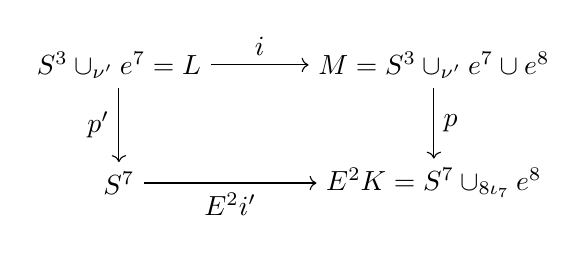
\begin{tikzpicture}[]
  \node (A) at (0,1.5) {$S^{3}\cup_{\nu'}e^7 = L$};
  \node (B) at (4,1.5) {$M = S^3\cup_{\nu'}e^7 \cup e^8$};
  \node (C) at (0,0) {$S^7$};
  \node (D) at (4,0) {$E^2 K = S^7\cup_{8\iota_7} e^8$};
  \draw[->] (A) -- node[above] {$i$} (B);
  \draw[->] (A) -- node[left] {$p'$} (C);
  \draw[->] (B) -- node[right] {$p$} (D);
  \draw[->] (C) -- node[below] {$E^2 i'$} (D);
\end{tikzpicture}


\noindent
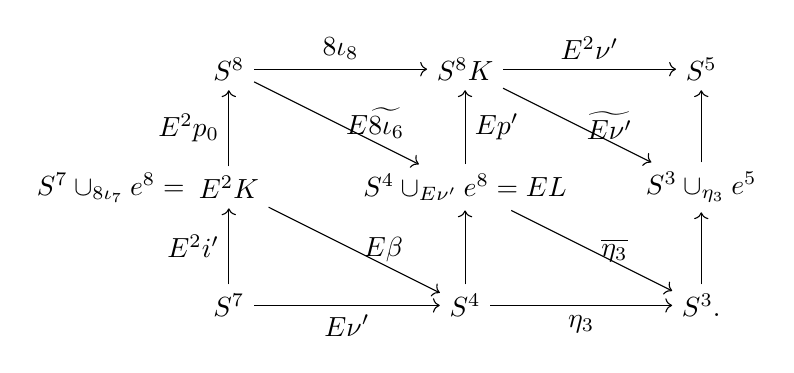
\begin{tikzpicture}[]
  \node (A) at (0,3) {$S^{8}$};
  \node (B) at (3,3) {$S^{8}K$};
  \node (C) at (6,3) {$S^5$};
  \node (D) at (0,1.5) {$E^{2}K$};
  \node (E) at (3,1.5) {$S^4\cup_{E\nu'}e^8=EL$};
  \node (F) at (6,1.5) {$S^3\cup_{\eta_3}e^5$};
  \node (G) at (0,0) {$S^7$};
  \node (H) at (3,0) {$S^4$};
  \node (I) at (6,0) {$S^3$.};
  \node (J) at (-1.5,1.5) {$S^7\cup_{8\iota_7}e^8 = $};
  \draw[->] (A) -- node[above] {$8\iota_8$} (B);
  \draw[->] (B) -- node[above] {$E^2\nu'$} (C);
  \draw[->] (A) -- node[right] {$E\widetilde{8\iota_6}$} (E);
  \draw[->] (B) -- node[right] {$\widetilde{E\nu'}$} (F);
  \draw[->] (D) -- node[left] {$E^2 p_0$} (A);
  \draw[->] (D) -- node[right] {$E\beta$} (H);
  \draw[->] (E) -- node[right] {$Ep'$} (B);
  \draw[->] (E) -- node[right] {$\overline{\eta_3}$} (I);
  \draw[->] (F) -- node[right] {} (C);
  \draw[->] (G) -- node[left] {$E^2 i'$} (D);
  \draw[->] (G) -- node[below] {$E\nu'$} (H);
  \draw[->] (H) -- node[left] {} (E);
  \draw[->] (H) -- node[below] {$\eta_3$} (I);
  \draw[->] (I) -- node[right] {} (F);
\end{tikzpicture}

\noindent
\(S^3\xlongleftarrow{\eta_3}
S^4 \xlongleftarrow{E\nu'}
S^7 \xlongleftarrow{\nu_7}
S^{10}\).

\noindent
\(S^3\xlongleftarrow{(Ei)^*\alpha}
S^4\cup_{E\nu'}e^8 = EL\xlongleftarrow{E\gamma'}
S^{11}\).




\end{paracol}

\begin{paracol}{2}

次に, \(\nu_{5}\) の coextension  \(\gamma\in\pi_{9}(K)\) を考える. \\
Prop1.7 より,
\(\beta\circ E\gamma\in 
\todai[1]{\nu',\,8\iota_{6},\,\nu_{6}}\) 
であり, \\
これは, (4.7), Prop5.15により, 
\(\pit{10}{3} = 0\) の部分集合である. \\
よって, \(\beta\circ E\gamma=0\) なので, 次の Toda bracket が定義できる. 
\[
\todai[1]{\eta_{3},\,E\beta,\,E^{2}\gamma}
\in \pi_{12}(S^{3}) / (\eta_{3}\circ E\pi_{11}(S^{3}) + [E^{3}K, S^{3}]\circ E^{3}\gamma) .
\]
(4.7) より,
\(\eta_{3}\circ E\pi_{11}(S^{3})=\eta_{3}\circ E\pi^{3}_{11}\) である. 
\begin{equation}\label{eq:6.4}
% \noindent
% \textbf{(6.4).}\
[E^{3}K, S^{3}] \circ E^{3}\gamma = 0,
\qquad
[E^{4}K, S^{4}] \circ E^{4}\gamma = \gen{\nu^{3}_{4}}.
\end{equation}

\noindent
\textbf{Proof.}\
\(\lambda\in [E^{3}K, S^{3}]\) を 考える. \\
\(\lambda\) は, ある元
\(\lambda'\in \pi_{8}(S^{3})\) の extension である. 
Prop1.7 より,
\[
-(\lambda\circ E^{3}\gamma)\ \in\ \todai[3]{\lambda',\,8\iota_{8},\,\nu_{8}}.
\]
\(\lambda'\circ 8\iota_{8}=8\lambda'=0\) なので, 
\(\lambda'\in \pi^{3}_{8} = \mathbb{Z}_2\gen{\nu'\circ\eta_6^2}\) である. \\
ゆえに, 
\(\lambda'
=y\,\nu' \circ \eta_6^{\,2},\ (y=0 \text{ or } 1) \) 
と表わせる. 
Prop1.7, (4.7), Prop5.8, 5.11 から,
\[
\begin{align*}
  \todai[3]{y\nu'\circ \eta_{6}^{2},\,8\iota_{8},\,\nu_{8}}
  \subset \todai[3]{y\nu', \eta_6^2\circ 8\iota_{8},\,\nu_{8}}\\
  = \todai[3]{y\nu', 0, \nu_8} 
  = y\nu'\circ E^3\pit{9}{3} + \pit{9}{3}\circ\nu_9 = 0 .
\end{align*}
\]
以上から, 
\(\lambda\circ E^{3}\gamma=0\) で, \eqref{eq:6.4} の第1式が示された. \\
第2式も同様に, 
\(\pit{10}{4}\circ \nu_{10} = \gen{\nu^{2}_{4}}\circ \nu_{10}
= \gen{\nu^{3}_{4}}\)
を用いればよい.
\qed

Toda bracket \(\todai[1]{\eta_{3},E\beta,E^{2}\gamma}\) 
の元を 1 つ選び, 
\[
\mu_{3}\in \todai[1]{\eta_{3},\,E\beta,\,E^{2}\gamma}
\in \pi_{12}(S^{3}) / (\eta_{3}\circ E\pi^{3}_{11})
\]
と書く. 
また, \(n\ge3\) に対し \(\mu_{n}:=E^{\,n-3}\mu_{3}\), 
\(\mu:=E^{\infty}\mu_{3}\) と書く. \\
これらの元 \(\mu_n\) は, 次の性質をもつ. 

\begin{lemma}\label{lem:6.5}
% \noindent
% \textbf{Lem6.5.}\
\(H(\mu_{3})=\sigma'''\), \quad
\(2\mu_{n}=2\mu=0\) (\(n\ge3\)) , 
\[
\mu_{n}\ \in\ \todai[n-4]{\eta_{n},\ 2\iota_{n+1},\ E^{\,n-4}\sigma'''}
\ +\ \gen{\nu^{3}_{n}},
\qquad (n\ge4).
\]
\end{lemma}

\noindent
\textbf{Proof.}\
Prop1.7 より, \(\eta_{3}\) の extension  \(\alpha\) と,
\(E\gamma\) の coextension  
\(\widetilde{\gamma}\in \pi_{11}(M)\) を用いて,\\
\(\mu_{3}=\alpha\circ E\widetilde{\gamma}\) と書ける. 
\[
\begin{align*}
  H(\mu_{3})
  & = H(\alpha\circ E\widetilde{\gamma})=H(\alpha)\circ E\widetilde{\gamma} 
  && \text{by Prop2.2}\\
  & = Ep^{\ast}\alpha'\circ E\widetilde{\gamma}
  = \alpha'\circ Ep_* E\coext{\gamma} 
  && \text{by (6.3)}\\
  & = \alpha'\circ E(p_*\coext{\gamma}) 
  = \alpha' \circ E^3\gamma 
  && \text{by (1.18)} .
\end{align*}
\]

\switchcolumn

\noindent
\(S^3\xlongleftarrow{\beta}
S^6\cup_{8\iota_6}e^7 = EK\xlongleftarrow{E\gamma}
S^{10}\).

\noindent
\textbf{Prop1.7.}\
\(\todai[n]{\alpha, E^n\beta, E^n\gamma}
= (-1)^n\gen{\overline{\alpha}\circ E^n\widetilde{\gamma}}\).

\noindent
\textbf{(4.7).}\
\(n\ge1, \ \alpha\in\pis{k+n}{S^m; 2},\ \gamma\in\pis{i}{S^j; 2}
\ \text{のとき, }\)\\
\(\alpha\circ E^n\pis{j}{S^k} = \alpha\circ E^n \pit{j}{k}
\subset \pit{j+n}{m},
\ \pis{j}{S^k}\circ\gamma = \pit{j}{k}\circ\gamma \subset\pit{i}{k}\ . \)\\
\(\text{さらに, }\ \alpha\circ E^n\beta=0,\ \beta\circ\gamma = 0 \ \text{のとき, }\)\\
\(\todai[n]{\alpha, E^n\beta, E^n\gamma}\ \text{は,}\
\alpha\circ E^n\pit{i+1}{k} + \pit{j+n+1}{m}\circ E^{n+1}\gamma\
\text{の coset で, }\pit{i+n+1}{m} \ \text{の部分集合である. }\)

\noindent
\textbf{Prop5.15.}\
\(\pi_9^2=\pi_{10}^3=\pi_{11}^4=0,\) \\
\(\pi^{5}_{12}=\mathbb Z_2\gen{\sigma'''},\) \
\(\pi^{6}_{13}=\mathbb Z_4\gen{\sigma''},\) \
\(\pi^{7}_{14}=\mathbb Z_8\gen{\sigma'},\) \
\(\pi^{8}_{15}=\mathbb Z\gen{\sigma_8}\oplus\mathbb Z\gen{E\sigma'},\) \\
\(\pi^{n}_{n+7}=\mathbb Z_{16}\gen{\sigma_n}\ (n\ge9),\) \
\((G_{7};2)=\mathbb Z_{16}\gen{\sigma}.\)

\noindent
\(S^3\xlongleftarrow{\lambda'}
S^8\xlongleftarrow{8\iota_8}
S^8\xlongleftarrow{\nu_8}
S^{11}\).

\noindent
\(S^3\xlongleftarrow{\lambda}
S^8\cup_{8\iota_8} e^9\xlongleftarrow{E^3\gamma}
S^{12}\).

\noindent
\textbf{Prop5.8.}\
\(\pi^{2}_{6}=\mathbb Z_4\gen{\eta_{2}\circ\nu'},\) \quad
\(\pi^{3}_{7}=\mathbb Z_2\gen{\nu'\circ\eta_6},\) \quad
\(\pi^{4}_{8}=\mathbb Z_2\gen{\nu_{4}\circ\eta_7}\oplus \mathbb Z_2\gen{E\nu'\circ\eta_7},\) \\
\(\pi^{5}_{9}=\mathbb Z_2\gen{\nu_{5}\circ\eta_8},\) \quad
\(\pi^{n}_{n+4}=0\ (n\ge6),\) \
\((G_{4};2)=0.\)

\noindent
\textbf{Prop5.11.}\
\(\pi^{2}_{8}=\mathbb Z_2\gen{\eta_{2}\circ\nu'\circ\eta_6^2},\)\quad 
\(\pi^{3}_{9}=0,\)\quad \(\pi^{4}_{10}=\mathbb Z_8\gen{\nu_{4}^2},\) \\
\(\pi^{n}_{n+6}=\mathbb Z_2\gen{\nu_n^2}\ (n\ge5),\) \
\((G_{6};2)=\mathbb Z_2\gen{\nu^2}.\)

\noindent
\textbf{Prop2.2.}\
$K,L$ を有限 cell complex とする. \\
$\alpha\in[EK, S^{m+1}], \ \beta\in[L,K], \ \gamma\in\pi_r(S^r)$ 
に対して, 次が成り立つ：\\
\(
H(\alpha\circ E\beta)\ =\ H(\alpha)\circ E\beta,
\)\\
\(
H(E\gamma\circ\alpha)\ =\ E(\gamma\wedge\gamma)\circ H(\alpha).
\)

\noindent
\textbf{(6.3).}\
\(H(\alpha)=E p^{\ast}\alpha',  
\quad \text{for some } \alpha'\in [E^{3}K, S^{5}],\)\\
\(H(Ei^{\ast}\alpha) = Ei^{\ast}H(\alpha) = (Ep')^{\ast}((E^3i')^{\ast}\alpha'),\)\\
\((E^3 i')^{\ast}\alpha' = x\,\nu_{5}\quad \text{for an odd integer }x.\)

\noindent
\textbf{(1.18).}\
\(p_*(\widetilde{\delta}) = E\delta,\qquad
\widetilde{\delta}\in[EV, X\cup_\gamma CW]:\
\delta\in [V,W]\) の coextension.

\noindent
\(\lambda\in[E^4 K, S^4]:\ \lambda'\in\pis{9}{S^4}\) の extension,\\
\(\lambda\circ E^4\gamma\in \todai[4]{\lambda', 8\iota_9, \nu_9}
\subset \todai[4]{y\alpha, \eta_7^2\circ 8\iota_9, \nu_9}\ni 0\).\\
\(y\alpha\circ E^4\pit{9}{3} + \pit{10}{4}\circ \nu_{10}
= \gen{\nu_4^2}\circ \nu_{10} = \gen{\nu_4^3}\).

\noindent
\(S^3\xlongleftarrow{\eta_3}
S^4\xlongleftarrow{E\beta}
S^7\cup_{8\iota_7}e^8 = E^2 K\xlongleftarrow{E^2\gamma}
S^{11}\).

\noindent
\(M = S^3\cup_{\beta}CEK\).

\noindent
\(S^3\xlongleftarrow{\alpha}
EM \xlongleftarrow{E\widetilde{\gamma}}
S^{12}\).

\noindent
\(S^5\xlongleftarrow{\alpha'}
S^8\cup_{8\iota_8}e^9 = E^3 K \xlongleftarrow{E^3\gamma}
S^{12}\).




\end{paracol}

\begin{paracol}{2}

\noindent
(6.3) により, 
\((E^3i')^*\alpha' = x\nu_5 .\)
これは, \(\alpha'\) が \(x\nu_5\) 
の extension であることを意味する. \\
\(\gamma\) は \(\nu_5\) の coextension なので, 
Prop1.7 から, 
\(\alpha'\circ E^3\gamma
\in \todai[3]{x\nu_5, 8\iota_8, \nu_8}\) である. \\
% ==== CHAPTER VI p.57 ====
Lem5.13 とProp1.2 から,
\[
x\iota_{5}\circ \sigma'''
\ \in\ x\iota_{5}\circ \todai[3]{\nu_{5},8\iota_{8},\nu_{8}}
\ \subset\ \todai[3]{x\nu_{5},8\iota_{8},\nu_{8}} .
\]
Lem5.13 の証明で見たように, 
最後の Toda bracket は単一元である. 
したがって,
\[
H(\mu_{3})=x\iota_{5}\circ \sigma'''.
\]
(5.14) より,
\(E:\pi^{5}_{12}\to \pi^{6}_{13}\) は単射であり, 
(2.1), (6.3), \(2\sigma'''=0\) から,
\[
E(x\iota_{5}\circ \sigma''')
=E(x\sigma''')=E\sigma''' .
\]
よって, \(x\iota_{5}\circ \sigma'''=\sigma'''\) であり, 
結局 \(H(\mu_{3})=\sigma'''\) である. 
\[
\begin{align*}
  2\mu_{3} 
  & = 2\iota_{3}\circ \mu_{3}
  \ \in\ 2\iota_{3}\circ \toda{\eta_{3},E\beta,E^{2}\gamma} 
  && \text{by Lem4.5}\\
  & = \toda{2\iota_{3},\eta_{3},E\beta}\circ (-E^{3}\gamma) 
  && \text{by Prop1.4}\\
  & \subset [E^{3}K, S^{3}]\circ E^{3}\gamma = 0 
  && \text{by (6.4)} .
\end{align*}
\]
したがって, \(n\ge3\) に対して, 
\(\,2\mu_{n}=2\mu=0\) である. 次に,
\[
\mu_{4}=-\,\mu_{4}\in -E\todai[1]{\eta_{3},E\beta,E^{2}\gamma}
\subset \toda{\,\eta_{4},E^{2}\beta,E^{3}\gamma\,}
\]
を考える. 
\(E^{2}\beta\in[E^{3}K, S^{5}]\) は, Lem5.4 により, 
\(E^{2}\nu'=2\nu_{5}\) の extension である. \\
\(\nu_{5}\circ 8\iota_{8}=8\nu_{5}=0\) なので, 
\(\nu_{5}\) の extension  \(\beta_{1}\in[E^{3}K, S^{5}]\) が存在する. \\
(2.1) により, \(2\iota_{5}\circ \beta_{1}\) は,
\(2\iota_{5}\circ \nu_{5}=2\nu_{5}\) の extension である. \\
したがって, 差
\(E^{2}\beta-2\iota_{5}\circ \beta_{1}\) は
\(2\nu_{5}-2\nu_{5}=0\) の extension である. \\
以上より, \(\beta_{2}\in\pi_{9}(S^{5})\) が存在して, 
\[
E^{2}\beta-2\iota_{5}\circ \beta_{1}=p_{0}^{\ast}\beta_{2}
\]
が成り立つ. 
ここで, \(p_{0}:E^{3}K\to S^{9}\) は shrinking map である. 
\begin{equation}\label{eq:6.5}
% \noindent
% \textbf{(6.5).}\
\begin{align*}
  \toda{\,\eta_{4},E^{2}\beta,E^{3}\gamma\,}
  & = \toda{\,\eta_{4},2\iota_{5}\circ \beta_{1},E^{3}\gamma\,}
  +\toda{\,\eta_{4},p_{0}^{\ast}\beta_{2},E^{3}\gamma\,}
  && \text{by Prop1.6}\\
  & \supset \toda{\eta_4, 2\iota_5, \beta_1\circ E^3\gamma}
  + \toda{\eta_4, \beta_2, p_0\circ E^3\gamma}
  && \text{by Prop1.2} .
\end{align*}
\end{equation}
Prop1.7 から,
\(\beta_{1}\circ E^{3}\gamma\in \todai[3]{\nu_{5},8\iota_{8},\nu_{8}}\) である. \\
Lem5.13 により,
\(\beta_{1}\circ E^{3}\gamma=\sigma''' .\)\\
また, (1.18) より, \(p_{0\ast}E^{3}\gamma=\nu_{9}\). 
% ==== CHAPTER VI p.58 ====
%  (前頁の続き： (6.5) の2項の扱い) 

\switchcolumn

\noindent
\textbf{(6.3).}\
\(H(\alpha)=E p^{\ast}\alpha',  
\quad \text{for some } \alpha'\in [E^{3}K, S^{5}],\)\\
\(H(Ei^{\ast}\alpha) = Ei^{\ast}H(\alpha) = (Ep')^{\ast}((E^3i')^{\ast}\alpha'),\)\\
\((E^3 i')^{\ast}\alpha' = x\,\nu_{5}\quad \text{for an odd integer }x.\)

\noindent
\textbf{Prop1.7.}\
\(\todai[n]{\alpha, E^n\beta, E^n\gamma}
= (-1)^n\gen{\overline{\alpha}\circ E^n\widetilde{\gamma}}\).

\noindent
\textbf{Lem5.13.}\
\(\todai[t]{\nu_5,8\iota_8,\nu_8},\ (0\leq t\leq3)\) 
は, ただ$1$つの元から成る. \\
この元を \(\sigma'''\) と書くと, 
\(H(\sigma''')=4\nu_9=\eta_9^3\) であり, \\
\(\pi_{12}^5=\mathbb{Z}_2\gen{\sigma'''}\)
である. 

\noindent
\textbf{Prop1.2.}\
\textbf{0).}\ $\alpha$, $\beta$, $\gamma$ のうち, いずれかが $0$ なら,
\(
\{\alpha,\ \Ex^n\beta,\ \Ex^n\gamma\}_n\equiv0.
\)\\
\textbf{i).}\ $\alpha\circ \Ex^n\beta=\beta\circ\gamma=0$ のとき,
\(
\{\alpha,\ \Ex^n\beta,\ \Ex^n\gamma\}_n\circ\Ex^{n+1}\delta\ \subset\ \{\alpha,\Ex^n \beta, \Ex^n(\gamma\circ\delta)\}_n.
\)\\
\textbf{ii).}\ $\alpha\circ \Ex^n\beta=\beta\circ\gamma\circ\delta=0$ のとき,
\(
\{\alpha,\ \Ex^n\beta,\ \Ex^n(\gamma\circ\delta)\}_n\ \subset\ \{\alpha,\ \Ex^n(\beta\circ\gamma),\ \Ex^n\delta\}_n .
\)\\
\textbf{iii).}\ $\alpha\circ\Ex^n\beta\circ\Ex^n\gamma=\gamma\circ\delta=0$ なら,
\(
\{\alpha\circ\Ex^n\beta,\ \Ex^n\gamma,\ \Ex^n\delta)\}_n\ \subset\ \{\alpha,\ \Ex^n(\beta\circ\gamma),\ \Ex^n\delta\}_n .
\)\\
\textbf{iv).}\ $\beta\circ\Ex^n\gamma=\gamma\circ\delta=0$ のとき,
\(
\alpha\circ\{\beta,\ \Ex^n\gamma,\ \Ex^n\delta\}_n\ \subset\ \{\alpha\circ\beta,\ \Ex^n\gamma,\ \Ex^n\delta\}_n .
\)

\noindent
\textbf{(5.14).}\
次の列は完全列である.\\
\(
0\to \pi^{5}_{12}\xrightarrow{E}\pi^{6}_{13}\xrightarrow{H}\pi^{11}_{13}\to0,
\quad
0\to \pi^{6}_{13}\xrightarrow{E}\pi^{7}_{14}\xrightarrow{H}\pi^{13}_{14}\to0 .
\)

\noindent
\textbf{(2.1).}\
\(k(\alpha\circ\beta) = \alpha\circ k\beta,\
k(\alpha\circ E\beta) = (k\alpha)\circ E\beta.\)

\noindent
\textbf{Lem4.5.}\
\(n=2,4,8\) のとき, 
\(E:\pis{i-1}{S^n-1}\to\pis{i}{S^n}\) は単射.\\ 
\(r\iota_{n-1}\circ\beta = r\beta,\ \beta\in\pis{i-1}{S^{n-1}}\).

\noindent
\textbf{Prop1.4.}\
\(\todai[n]{\alpha, E^n\beta, E^n\gamma}\circ E^{n+1}\delta
= (-1)^{n+1}(\alpha\circ E^n\toda{\beta, \gamma, \delta})\).

\noindent
\textbf{(6.4).}\
\([E^{3}K, S^{3}] \circ E^{3}\gamma = 0, \
[E^{4}K, S^{4}] \circ E^{4}\gamma = \gen{\nu^{3}_{4}}.\)

\noindent
\textbf{Lem5.4.}\
ある元 \(\nu_{4}\in \pi^{4}_{7}\) が存在して, 次を満たす. \\
\(H(\nu_{4})=\iota_7,\ 2E \nu_{4}=E^{2}\nu' .\)

\noindent
\textbf{Prop1.6}\
$\alpha,\alpha'\in[\Ex^n Y, Z]$, $\beta,\beta'\in[X, Y]$, 
$\gamma,\gamma'\in[W, X]$ とする. \\
$n\ge 1$ または, $W=\Ex W'$ のとき,\\
\(
\{\alpha,\Ex^n\beta,\Ex^n\gamma\}_n
+
\{\alpha,\Ex^n\beta,\Ex^n\gamma'\}_n
\ \supset\
\{\alpha,\Ex^n\beta,\Ex^n(\gamma+\gamma')\}_n.
\)\\
$n\ge 1$ または, $\gamma=\Ex\gamma' \ (X=\Ex X,\ W=\Ex W')$ のとき,\\
\(
\{\alpha,\Ex^n\beta,\Ex^n\gamma\}_n
+
\{\alpha,\Ex^n\beta',\Ex^n\gamma\}_n
\ =\
\{\alpha,\Ex^n(\beta+\beta'),\Ex^n\gamma\}_n.
\)\\
$n\ge 1$ または,
$\beta=\Ex\beta',\ \gamma=\Ex\gamma' \ (Y=\Ex Y',\ X=\Ex X',\ W=\Ex W')$ のとき,\\
\(
\{\alpha,\Ex^n\beta,\Ex^n\gamma\}_n
+
\{\alpha',\Ex^n\beta,\Ex^n\gamma\}_n
\ \supset\
\{\alpha+\alpha',\Ex^n\beta,\Ex^n\gamma\}_n.
\)

\noindent
\textbf{(1.18).}\
\(p_*(\widetilde{\delta}) = E\delta,\quad
\widetilde{\delta}\in[EV, X\cup_\gamma CW]:\
\delta\in [V,W]\) の coextension.

\noindent
\(S^8\longrightarrow 
S^8\cup_{8\iota_8}e^9 = E^3 K \xlongrightarrow{p_0}
S^9\).\\
\(\pis{9}{S^5}\longrightarrow
[E^3 K, S^5]\longrightarrow
\pis{8}{S^5}\)\\
\({}^\exists \beta_2 \longmapsto 
E^2\beta - 2\iota_5\circ\beta_1 \longmapsto
2\nu_5 - 2\nu_5 = 0\)




\end{paracol}

\begin{paracol}{2}

\noindent
\(\pi_{9}(S^{5})\) は有限群なので, 
\(r\equiv1\pmod 8\) を満たす整数 \(r\) が存在して, 
\(r\beta_{2}\in \pi^{5}_{9}\). \\
Prop5.8, 5.9, (5.9) より, 
\(\pi^{5}_{9}\cong\mathbb Z_{2}\) 
の生成元 \(\nu_{5}\circ \eta_{8}\) について,
\[
\eta_{4}\circ \nu_{5}\circ \eta_{8}
  \;=\; E\nu'\circ \eta_{7}^{\,2}\ \ne 0 .
\]
\(\eta_{4}\circ r\beta_{2}=0\) なので,
\(r\beta_{2}=0\) である. 
Prop1.2 より,
\[
\toda{\,\eta_{4},\ \beta_{2},\ r\nu_{9}\,}
\subset \toda{\,\eta_{4},\ r\beta_{2},\ \nu_{9}\,}
= \toda{\eta_4, 0, \nu_9}
\equiv 0 .
\]
(4.7) とProp5.11 から, Toda bracket 
\[
\toda{\,\eta_{4},\ \beta_{2},\ p_{0\ast}E^{3}\gamma\,}
= \toda{\,\eta_{4},\ \beta_{2},\ \nu_{9}\,}
= \toda{\eta_4, \beta_2, r\nu_9},\quad
\toda{\eta_4, 0, \nu_9}
\]
は, どちらも次の部分群の coset である. 
\[
\,\eta_{4}\circ \pi_{13}(S^{5}) + \pit{10}{4}\circ\nu_{10}
= \eta_4\circ\pis{13}{S^5} + \gen{\nu^{3}_{4}} .
\] 
よって,
\[
\toda{\eta_4, \beta_2, p_{0*}E^3\gamma}
=\eta_4\circ\pis{13}{S^5} + \gen{\nu_4^3}.
\]
さらに, (4.7) と (6.4) から,
\(\toda{\,\eta_{4},\ E^{2}\beta,\ E^{3}\gamma\,}\)
は, 
\(\eta_{4}\circ \pi_{13}(S^{5})
+\gen{\nu^{3}_{4}}\) の coset である. \\
よって, \eqref{eq:6.5} の包含はイコールであり, 
\[
\mu_{4}\ \in\ \toda{\,\eta_{4},\ E^{2}\beta,\ E^{3}\gamma\,}
 \ =\ \toda{\,\eta_{4},\ 2\iota_{5},\ \sigma^{\prime\prime\prime}\,}\ +\ \gen{\nu^{3}_{4}}\ .
\]
Prop1.3 を用いれば,
\[
\begin{align*}
\mu_{n} = (-1)^{n-4}E^{\,n-4}\mu_{4}
& \in (-1)^{n-4}E^{\,n-4}(\toda{\,\eta_{4},2\iota_{5},\sigma'''\,}
  +\gen{\nu^{3}_{4}})\\
& \subset \todai[n-4]{\eta_{n},2\iota_{n+1},E^{\,n-4}\sigma'''}
  +\gen{\nu^{3}_{n}} .
\end{align*}
\]
これで, Lem\ref{lem:6.5} は示された. 
\qed

\bigskip
\paragraph{iv). The element \(\varepsilon'\).}

(4.7) とProp5.11 より,
\(\nu'\circ\nu_6\) と \(\nu'\circ2\nu_6\) は,
\(\pit{9}{3} = 0\) の元である. \\
よって, 
\(\nu'\circ 2\nu_{6}=\nu'\circ \nu_{6}=0 .\)\\
また, \(E^{3}\nu'=2\nu_{6}\) なので,  Toda bracket 
\[
\todai[3]{\nu',\ 2\nu_{6},\ \nu_{9}}
\]
が定義され, (4.7) とProp5.15 より,
\(\,\nu'\circ E^{3}\pi^{3}_{10}+\pi^{3}_{10}\circ \nu_{10}=0\) の coset である. \\
したがって, Toda bracket は単一元から成り, それを
\[
\varepsilon'\ :=\ \todai[3]{\nu',\ 2\nu_{6},\ \nu_{9}}
\ \in\ \pi_{13}(S^{3})
\]
と置く. 

\switchcolumn

\noindent
\textbf{Prop5.8.}\
\(\pi^{2}_{6}=\mathbb Z_4\gen{\eta_{2}\circ\nu'},\) \quad
\(\pi^{3}_{7}=\mathbb Z_2\gen{\nu'\circ\eta_6},\) \quad
\(\pi^{4}_{8}=\mathbb Z_2\gen{\nu_{4}\circ\eta_7}\oplus \mathbb Z_2\gen{E\nu'\circ\eta_7},\) \\
\(\pi^{5}_{9}=\mathbb Z_2\gen{\nu_{5}\circ\eta_8},\) \quad
\(\pi^{n}_{n+4}=0\ (n\ge6),\) \
\((G_{4};2)=0.\)

\noindent
\textbf{Prop5.9.}\
\(\pi^{2}_{7}=\mathbb Z_2\gen{\eta_{2}\circ\nu'\circ\eta_6},\) \quad
\(\pi^{3}_{8}=\mathbb Z_2\gen{\nu'\circ\eta_6^2},\) \quad
\(\pi^{4}_{9}=\mathbb Z_2\gen{\nu_{4}\circ\eta_7^2}\oplus \mathbb Z_2\gen{E\nu'\circ\eta_7^2},\) \\
\(\pi^{5}_{10}=\mathbb Z_2\gen{\nu_{5}\circ\eta_8^2},\) \quad
\(\pi^{6}_{11}=\mathbb Z_2\gen{\Delta(\iota_{13})},\) \quad
\(\pi^{n}_{n+5}=0\ (n\ge7),\) \
\((G_{5};2)=0.\)

\noindent
\textbf{(5.9).}\
\(\eta_3\circ \nu_4= \nu'\circ \eta_6,\
\eta_n\circ \nu_{n+1}=0\ (n\ge5),\
\nu_n\circ \eta_{n+3}=0\ (n\ge6)\)

\noindent
\textbf{Prop1.2.}\
\textbf{0).}\ $\alpha$, $\beta$, $\gamma$ のうち, いずれかが $0$ なら,
\(
\{\alpha,\ \Ex^n\beta,\ \Ex^n\gamma\}_n\equiv0.
\)\\
\textbf{i).}\ $\alpha\circ \Ex^n\beta=\beta\circ\gamma=0$ のとき,
\(
\{\alpha,\ \Ex^n\beta,\ \Ex^n\gamma\}_n\circ\Ex^{n+1}\delta\ \subset\ \{\alpha,\Ex^n \beta, \Ex^n(\gamma\circ\delta)\}_n.
\)\\
\textbf{ii).}\ $\alpha\circ \Ex^n\beta=\beta\circ\gamma\circ\delta=0$ のとき,
\(
\{\alpha,\ \Ex^n\beta,\ \Ex^n(\gamma\circ\delta)\}_n\ \subset\ \{\alpha,\ \Ex^n(\beta\circ\gamma),\ \Ex^n\delta\}_n .
\)\\
\textbf{iii).}\ $\alpha\circ\Ex^n\beta\circ\Ex^n\gamma=\gamma\circ\delta=0$ なら,
\(
\{\alpha\circ\Ex^n\beta,\ \Ex^n\gamma,\ \Ex^n\delta)\}_n\ \subset\ \{\alpha,\ \Ex^n(\beta\circ\gamma),\ \Ex^n\delta\}_n .
\)\\
\textbf{iv).}\ $\beta\circ\Ex^n\gamma=\gamma\circ\delta=0$ のとき,
\(
\alpha\circ\{\beta,\ \Ex^n\gamma,\ \Ex^n\delta\}_n\ \subset\ \{\alpha\circ\beta,\ \Ex^n\gamma,\ \Ex^n\delta\}_n .
\)

\noindent
\textbf{(4.7).}\
\(n\ge1, \ \alpha\in\pis{k+n}{S^m; 2},\ \gamma\in\pis{i}{S^j; 2}
    \ \text{のとき, }\)\\
\(\alpha\circ E^n\pis{j}{S^k} = \alpha\circ E^n \pit{j}{k}
  \subset \pit{j+n}{m},
  \ \pis{j}{S^k}\circ\gamma = \pit{j}{k}\circ\gamma \subset\pit{i}{k}\ . \)\\
\(\text{さらに, }\ \alpha\circ E^n\beta=0,\ \beta\circ\gamma = 0 \ \text{のとき, }\)\\
\(\todai[n]{\alpha, E^n\beta, E^n\gamma}\ \text{は,}\
  \alpha\circ E^n\pit{i+1}{k} + \pit{j+n+1}{m}\circ E^{n+1}\gamma\
  \text{の coset で, }\pit{i+n+1}{m} \ \text{の部分集合である. }\)

\noindent
\textbf{Prop5.11.}\
\(\pi^{2}_{8}=\mathbb Z_2\gen{\eta_{2}\circ\nu'\circ\eta_6^2},\)\quad 
\(\pi^{3}_{9}=0,\)\quad \(\pi^{4}_{10}=\mathbb Z_8\gen{\nu_{4}^2},\) \\
\(\pi^{n}_{n+6}=\mathbb Z_2\gen{\nu_n^2}\ (n\ge5),\) \
\((G_{6};2)=\mathbb Z_2\gen{\nu^2}.\)

\noindent
\textbf{(6.4).}\
\([E^{3}K, S^{3}] \circ E^{3}\gamma = 0, \
[E^{4}K, S^{4}] \circ E^{4}\gamma = \gen{\nu^{3}_{4}}.\)

\noindent
\textbf{(6.5).}\
\(\toda{\,\eta_{4},E^{2}\beta,E^{3}\gamma\,}
 = \toda{\,\eta_{4},2\iota_{5}\circ \beta_{1},E^{3}\gamma\,}
+\toda{\,\eta_{4},p_{0}^{\ast}\beta_{2},E^{3}\gamma\,},\
\text{by Prop1.6}\)\\
\(\supset \toda{\eta_4, 2\iota_5, \beta_1\circ E^3\gamma}
+ \toda{\eta_4, \beta_2, p_0\circ E^3\gamma},\
\text{by Prop1.2} .\)

\noindent
\textbf{Prop1.3.}\
\(-E\todai[n]{\alpha, E^n\beta, E^n\gamma}
\subset \todai[n+1]{E\alpha, E^{n+1}\beta, E^{n+1}\gamma}\).

\noindent
\textbf{Lem6.5.}\
\(H(\mu_{3})=\sigma'''\), \quad
\(2\mu_{n}=2\mu=0\) (\(n\ge3\)) , \\
\(
\mu_{n}\ \in\ \todai[n-4]{\eta_{n},\ 2\iota_{n+1},\ E^{\,n-4}\sigma'''}
\ +\ \gen{\nu^{3}_{n}},
\quad (n\ge4).
\)

\noindent
\textbf{Prop5.15.}\
\(\pi_9^2=\pi_{10}^3=\pi_{11}^4=0,\) \\
\(\pi^{5}_{12}=\mathbb Z_2\gen{\sigma'''},\) \
\(\pi^{6}_{13}=\mathbb Z_4\gen{\sigma''},\) \
\(\pi^{7}_{14}=\mathbb Z_8\gen{\sigma'},\) \
\(\pi^{8}_{15}=\mathbb Z\gen{\sigma_8}\oplus\mathbb Z\gen{E\sigma'},\) \\
\(\pi^{n}_{n+7}=\mathbb Z_{16}\gen{\sigma_n}\ (n\ge9),\) \
\((G_{7};2)=\mathbb Z_{16}\gen{\sigma}.\)






\end{paracol}

\begin{paracol}{2}

\begin{lemma}\label{lem:6.6}
% \noindent
% \textbf{Lem6.6.}\
\(H(\varepsilon')=\varepsilon_{5}\), \quad
\(2\varepsilon'=\eta_{3}^{\,2}\varepsilon_{5}\), \quad
\(E^{2}\varepsilon'\) は $2$ で割れる. 
\end{lemma}

\noindent
\textbf{Proof.}\
Prop2.3 と (5.3) より,
\[
H(\varepsilon')\in H\todai[3]{\nu',2\nu_{6},\nu_{9}}
 \subset \todai[3]{H(\nu'),\,2\nu_{6},\,\nu_{9}}
 = \todai[3]{\eta_{5},\,2\nu_{6},\,\nu_{9}} .
\]
(6.1) から, \(\varepsilon_{5}\in \todai[3]{\eta_{5},2\nu_{6},\nu_{9}} .\)\\
さらに, (4.7), Prop5.15, Prop5.9, (5.9) より,
\(\todai[3]{\eta_{5},2\nu_{6},\nu_{9}}\) は,
\[
\eta_{5}\circ E^{3}\pi^{3}_{10}+\pi^{5}_{10}\circ \nu_{10}
= 0+\gen{\nu_{5}\circ \eta_{8}\circ \nu_{10}}=0
\]
の coset で, 単一元から成る. 
よって, \(H(\varepsilon')=\varepsilon_{5}\)である. \\
同様に \(\todai[3]{\eta_{3}^{3},2\nu_{6},\nu_{9}}\) 
も単一元から成る. \\
% ==== CHAPTER VI p.59 ====
よって, 次の２つの関係から,
\(2\varepsilon'=\eta_{3}^{\,2}\circ\varepsilon_{5}\) が従う. 
\[
\begin{align*}
2\varepsilon'
& = 2\iota_{3}\circ \varepsilon'
\in 2\iota_{3}\circ \todai[3]{\nu',2\nu_{6},\nu_{9}}
&& \text{by Lem4.5}\\
& \subset \todai[3]{2\iota_{3}\circ\nu',2\nu_{6}, \nu_{9}}
&& \text{by Prop1.2}\\
& = \todai[3]{2\nu',2\nu_{6},\nu_{9}}
= \todai[3]{\eta_{3}^{\,2},2\nu_{6},\nu_{9}}
&& \text{by Lem4.5, (5.3)},\\
\eta_{3}^{\,2}\circ \varepsilon_{5}
& \in \eta_{3}^{\,2}\circ \todai[3]{\eta_{5},2\nu_{6},\nu_{9}}
&& \text{by (6.1)}\\
& \subset \todai[3]{\eta_{3}^{\,2},2\nu_{6},\nu_{9}}
&& \text{by Prop1.2}.
\end{align*}
\]
\[
\todai[5]{\nu_{5},\,2\nu_{8},\,\nu_{11}},\qquad
\todai[5]{\nu_{5},\,4\nu_{8},\,\nu_{11}}
\]
は,  (4.7) , Prop5.15 より, 
\(\nu_{5}\circ E^{5}\pi^{3}_{10}+\pi^{5}_{12}\circ \nu_{12}=\gen{\sigma^{\prime\prime\prime}\circ \nu_{12}}\)
の coset である. \\
Prop1.2, 1.3 と Lem5.4 を用いると,
\[
\begin{align*}
E^{2}\varepsilon'
& \in E^{2}\todai[3]{\nu',2\nu_{6},\nu_{9}}
\subset \todai[5]{E^{2}\nu',\,2\nu_{8},\,\nu_{11}} \\
& = \todai[5]{2\nu_{5},2\nu_{8},\nu_{11}}
\subset \todai[5]{\nu_{5},4\nu_{8},\nu_{11}},\\
2\todai[5]{\nu_{5},2\nu_{8},\nu_{11}}
& = \todai[5]{\nu_{5},8\nu_{8},\nu_{11}}\circ 2\iota_{15}\\
& \subset \todai[5]{\nu_{5},2\nu_{8},2\nu_{11}}
\subset \todai[5]{\nu_{5},4\nu_{8},\nu_{11}}.
\end{align*}
\]
したがって, 
\(\alpha\in\todai[5]{\nu_{5},2\nu_{8},\nu_{11}}\) 
に対して, 整数 \(x\) が存在して,
\[
2\alpha
=E^{2}\varepsilon' + x\,\sigma^{\prime\prime\prime}\circ \nu_{12}.
\]
(6.2) より, ある整数 \(y\) が存在して, 
\[
\sigma^{\prime\prime\prime}\circ \nu_{12}
=\eta_{5}^{\,2}\circ \varepsilon_{7}+4y\,\nu_{5}\circ E\sigma' 
= 2(E^2 \varepsilon' + 2y\nu_5\circ E\sigma') .
\]
\[
2\alpha = 
E^2\varepsilon' + 
2(xE^2\varepsilon' + 2xy\nu_5\circ E\sigma').
\]
\begin{equation}\label{eq:6.6}
E^{2}\varepsilon'
=2(\,\alpha + x\,E^{2}\varepsilon' + 2xy\,\nu_{5}\circ E\sigma'\,).
\end{equation}
これで, Lem\ref{lem:6.6} が示された. 
\qed

\switchcolumn

\noindent
\textbf{Prop2.3.}\
$n\ge1$ とし, 元
\(
\alpha\in[E^nK, S^{m+1}],\
\beta\in[L, K],\
\gamma\in[M, L]
\)
が, \\
条件
\(
\alpha\circ E^n\beta=0,\ \beta\circ\gamma=0
\)
を満たすと仮定する. このとき,\\
\(
H\!\bigl(\,\{\,\alpha,\ E^n\beta,\ E^n\gamma\,\}_n\bigr)\ \subset\
\{\,H(\alpha),\ E^n\beta,\ E^n\gamma\,\}_n .
\)

\noindent
\textbf{(5.3).}\
\(\nu'\in\pi_6^3,\ H(\nu')=\eta_5,\ 2\nu'=\eta_3\circ\eta_4\circ\eta_5 .\)

\noindent
\textbf{(6.1).}\ 
\(\text{次の Toda bracket は } \varepsilon_n \text{ を含んでいる. }\quad\)\\
\(n\ge4,\ 0\le t\le n-2\) に対して, 
\(
\todai[t]{\eta_n,\ 2\nu_{n+1},\ \nu_{n+4}},
\)\\
\(n\ge5,\ 0\le t\le n-5\) に対して, \\
\(
\todai[t]{\eta_n, \nu_{n+1}, 2\nu_{n+4}},\
\todai[t]{\eta_n, 2\iota_{n+1}, \nu_{n+1}^2},\
\todai[t]{\eta_n,\ \nu_{n+1}^{2},\ \iota_{n+7}} .
\)

\noindent
\textbf{(4.7).}\
\(n\ge1, \ \alpha\in\pis{k+n}{S^m; 2},\ \gamma\in\pis{i}{S^j; 2}
    \ \text{のとき, }\)\\
\(\alpha\circ E^n\pis{j}{S^k} = \alpha\circ E^n \pit{j}{k}
  \subset \pit{j+n}{m},
  \ \pis{j}{S^k}\circ\gamma = \pit{j}{k}\circ\gamma \subset\pit{i}{k}\ . \)\\
\(\text{さらに, }\ \alpha\circ E^n\beta=0,\ \beta\circ\gamma = 0 \ \text{のとき, }\)\\
\(\todai[n]{\alpha, E^n\beta, E^n\gamma}\ \text{は,}\
  \alpha\circ E^n\pit{i+1}{k} + \pit{j+n+1}{m}\circ E^{n+1}\gamma\
  \text{の coset で, }\pit{i+n+1}{m} \ \text{の部分集合である. }\)

\noindent
\textbf{Prop5.15.}\
\(\pi_9^2=\pi_{10}^3=\pi_{11}^4=0,\) \\
\(\pi^{5}_{12}=\mathbb Z_2\gen{\sigma'''},\) \
\(\pi^{6}_{13}=\mathbb Z_4\gen{\sigma''},\) \
\(\pi^{7}_{14}=\mathbb Z_8\gen{\sigma'},\) \
\(\pi^{8}_{15}=\mathbb Z\gen{\sigma_8}\oplus\mathbb Z\gen{E\sigma'},\) \\
\(\pi^{n}_{n+7}=\mathbb Z_{16}\gen{\sigma_n}\ (n\ge9),\) \
\((G_{7};2)=\mathbb Z_{16}\gen{\sigma}.\)

\noindent
\textbf{Prop5.9.}\
\(\pi^{2}_{7}=\mathbb Z_2\gen{\eta_{2}\circ\nu'\circ\eta_6},\) \quad
\(\pi^{3}_{8}=\mathbb Z_2\gen{\nu'\circ\eta_6^2},\) \quad
\(\pi^{4}_{9}=\mathbb Z_2\gen{\nu_{4}\circ\eta_7^2}\oplus \mathbb Z_2\gen{E\nu'\circ\eta_7^2},\) \\
\(\pi^{5}_{10}=\mathbb Z_2\gen{\nu_{5}\circ\eta_8^2},\) \quad
\(\pi^{6}_{11}=\mathbb Z_2\gen{\Delta(\iota_{13})},\) \quad
\(\pi^{n}_{n+5}=0\ (n\ge7),\) \
\((G_{5};2)=0.\)

\noindent
\textbf{(5.9).}\
\(\eta_3\circ \nu_4= \nu'\circ \eta_6,\
\eta_n\circ \nu_{n+1}=0\ (n\ge5),\
\nu_n\circ \eta_{n+3}=0\ (n\ge6)\)

\noindent
\textbf{Lem4.5.}\
\(n=2,4,8\) のとき, 
\(E:\pis{i-1}{S^n-1}\to\pis{i}{S^n}\) は単射.\\ 
\(r\iota_{n-1}\circ\beta = r\beta,\ \beta\in\pis{i-1}{S^{n-1}}\).

\noindent
\textbf{Prop1.2.}\
\textbf{0).}\ $\alpha$, $\beta$, $\gamma$ のうち, いずれかが $0$ なら,
\(
\{\alpha,\ \Ex^n\beta,\ \Ex^n\gamma\}_n\equiv0.
\)\\
\textbf{i).}\ $\alpha\circ \Ex^n\beta=\beta\circ\gamma=0$ のとき,
\(
\{\alpha,\ \Ex^n\beta,\ \Ex^n\gamma\}_n\circ\Ex^{n+1}\delta\ \subset\ \{\alpha,\Ex^n \beta, \Ex^n(\gamma\circ\delta)\}_n.
\)\\
\textbf{ii).}\ $\alpha\circ \Ex^n\beta=\beta\circ\gamma\circ\delta=0$ のとき,
\(
\{\alpha,\ \Ex^n\beta,\ \Ex^n(\gamma\circ\delta)\}_n\ \subset\ \{\alpha,\ \Ex^n(\beta\circ\gamma),\ \Ex^n\delta\}_n .
\)\\
\textbf{iii).}\ $\alpha\circ\Ex^n\beta\circ\Ex^n\gamma=\gamma\circ\delta=0$ なら,
\(
\{\alpha\circ\Ex^n\beta,\ \Ex^n\gamma,\ \Ex^n\delta)\}_n\ \subset\ \{\alpha,\ \Ex^n(\beta\circ\gamma),\ \Ex^n\delta\}_n .
\)\\
\textbf{iv).}\ $\beta\circ\Ex^n\gamma=\gamma\circ\delta=0$ のとき,
\(
\alpha\circ\{\beta,\ \Ex^n\gamma,\ \Ex^n\delta\}_n\ \subset\ \{\alpha\circ\beta,\ \Ex^n\gamma,\ \Ex^n\delta\}_n .
\)

\noindent
\textbf{Prop1.3.}\
\(-E\todai[n]{\alpha, E^n\beta, E^n\gamma}
\subset \todai[n+1]{E\alpha, E^{n+1}\beta, E^{n+1}\gamma}\).

\noindent
\textbf{Lem5.4.}\
ある元 \(\nu_{4}\in \pi^{4}_{7}\) が存在して, 次を満たす. \\
\(H(\nu_{4})=\iota_7,\ 2E \nu_{4}=E^{2}\nu' .\)

\noindent
\textbf{(6.2).}\ 
\(\sigma'''\circ \nu_{12}\ \equiv\ \eta_5^{\,2}\circ \varepsilon_7
\mod{4(\nu_5\circ E\sigma')} .\)







\end{paracol}

\begin{paracol}{2}

\paragraph{v). The elements \(\zeta_{n}\).}

次の Toda bracket を考える. 
\[
\todai[1]{\nu_{5},\,8\iota_{8},\,E\sigma'}
\ \subset\ \pi^{5}_{16}
\]
ここで, \(\nu_{5}\circ 8\iota_{8}=8\nu_{5}=0\) であり, 
(2.1) により, 
\(E(8\iota_{7}\circ \sigma')=8E\sigma'=0\) である. \\
Lem4.5 より, \(8\iota_{7}\circ \sigma'=0\) である. \\
したがって, 上の Toda bracket は定義され,
\[
\nu_{5}\circ E\pi^{7}_{15}+\pi^{7}_{9}\circ E^{2}\sigma'
\] 
の coset である. 
Prop5.8 と Lem5.14 から,
\[
\pi^{5}_{9}\circ E^{2}\sigma'
=\gen{\nu_{5}\circ \eta_{8}\circ 2\sigma_{9}}
=\gen{\eta_{5}\circ 2\eta_{8}\circ \sigma_{9}} = 0 .
\]
この Toda bracket の元の一つを,
\[
\zeta_{5}\ \in\ \todai[1]{\nu_{5},\,8\iota_{8},\,E\sigma'}
\ \in\ \pi^{5}_{16}/\bigl(\nu_{5}\circ E\pi^{7}_{15}\bigr)
\]
と書く. さらに,
\[
\zeta_{n}:=E^{\,n-5}\zeta_{5}\quad(n\ge5),\qquad
\zeta:=E^{\infty}\zeta_{5}.
\]

\begin{lemma}\label{lem:6.7}
% \noindent
% \textbf{Lem6.7.}\
\(H(\zeta_{5})=8\sigma_{9}\), \quad
\(4\zeta_{5}\equiv \eta_{5}^{\,2}\circ \mu_{7}\ \ (\mathrm{mod}\ \nu_{5}\circ E\pi^{7}_{15})\).\\
\(4E\pit{15}{7} = 0\) ならば, \(n\ge5\) に対して, \(8\zeta_n=8\zeta=0\).
\end{lemma}

% ==== CHAPTER VI p.60 ====

\noindent
\textbf{Proof.}\
Prop2.6 より,
\[
H(\zeta_{5})\in H\todai[1]{\nu_{5},8\iota_{8},E\sigma'}
 = \Delta^{-1}(\nu_{4}\circ 8\iota_{7})\circ E^{2}\sigma' .
\]
(5.8) から,
\[
\pm\,\Delta(4\iota_{9})=4(2\nu_{4}-E\nu')
=8\nu_{4}=\nu_{4}\circ8\iota_{7} .
\]
したがって, Lem5.14 により, 
\[
H\todai[1]{\nu_{5},8\iota_{8},E\sigma'}\ \ni\ 
4\iota_9\circ E^2\sigma' = 8\sigma_9 .
\]
\(H\todai[1]{\nu_{5},8\iota_{8},E\sigma'}\) は,
\(H(\nu_{5}\circ E\pi^{7}_{15})=HE(\nu_{4}\circ \pi^{7}_{15})=0\)
の coset なので, \\
結局 \(H(\zeta_{5})=8\sigma_{9}\) を得る. \\
\(\todai[1]{\nu_5, 8\iota_8, E\sigma'}\) 
と同様の方法で, \\
\(\todai[1]{\nu_{5},8\iota_{8},E^{2}\sigma''}\) 
は, \(\nu_5\circ E\pit{15}{7}\) の coset, \\
\(\todai[1]{2\nu_{5},4\iota_{8},E^{3}\sigma'''}\)
は, \(2\nu_5\circ E\pit{15}{7} = \nu_5\circ2E\pit{15}{7}\) の coset である.

\switchcolumn

\noindent
\textbf{(2.1).}\
\(k(\alpha\circ\beta) = \alpha\circ k\beta,\
k(\alpha\circ E\beta) = (k\alpha)\circ E\beta.\)

\noindent
\textbf{Lem4.5.}\
\(n=2,4,8\) のとき, 
\(E:\pis{i-1}{S^n-1}\to\pis{i}{S^n}\) は単射.\\ 
\(r\iota_{n-1}\circ\beta = r\beta,\ \beta\in\pis{i-1}{S^{n-1}}\).

\noindent
\textbf{Prop5.8.}\
\(\pi^{2}_{6}=\mathbb Z_4\gen{\eta_{2}\circ\nu'},\) \quad
\(\pi^{3}_{7}=\mathbb Z_2\gen{\nu'\circ\eta_6},\) \quad
\(\pi^{4}_{8}=\mathbb Z_2\gen{\nu_{4}\circ\eta_7}\oplus \mathbb Z_2\gen{E\nu'\circ\eta_7},\) \\
\(\pi^{5}_{9}=\mathbb Z_2\gen{\nu_{5}\circ\eta_8},\) \quad
\(\pi^{n}_{n+4}=0\ (n\ge6),\) \
\((G_{4};2)=0.\)

\noindent
\textbf{Lem5.14.}\
\(\sigma_{8}\in\pi^{8}_{15}\ , \ \sigma'\in\pi^{7}_{14}\ , \ \sigma''\in\pi^{6}_{13}\) 
が存在して, 次を満たす. \\
\(H(\sigma_{8})=\iota_{15} \ ,\quad 2E\sigma_{8}=E^{2}\sigma',\)\\
\(H(\sigma')=\eta_{13} \ ,\quad 2\sigma'=E\sigma'',\)\\
\(H(\sigma'')=\eta_{11}^2 \ ,\quad 2\sigma''=E\sigma''' .\)

\noindent
\textbf{Prop2.6.}\
\(H\todai[1]{E\alpha, E\beta, E\gamma} 
= -\Delta^{-1}(\alpha\circ\beta)\circ E^2\gamma.\)

\noindent
\textbf{(5.8).}\
\(\Delta(\iota_9)=\pm(2\nu_4-E\nu')  \ (=\pm[\iota_4, \iota_4]) .\)

\noindent
\(\pit{9}{5}\circ E^3\sigma'' 
= \gen{\nu_5\circ\eta_8\circ E^3\sigma''}
= \gen{\nu_5\circ\eta_8\circ 4\sigma_9} = 0.\)\\
\(\pit{9}{5}\circ E^4\sigma''' 
= \gen{\nu_5\circ\eta_8\circ E^4\sigma'''}
= \gen{\nu_5\circ\eta_8\circ 8\sigma_9} = 0.\)




\end{paracol}

\begin{paracol}{2}

\noindent
Prop1.2 により, 
\[
\begin{align*}
2\zeta_{5}\in\todai[1]{\nu_{5},8\iota_{8},E\sigma'}\circ 2\iota_{16}
& \subset \todai[1]{\nu_{5},8\iota_{8},2E\sigma'}\\
& = \todai[1]{\nu_{5},8\iota_{8},E^{2}\sigma''}, \\
\todai[1]{2\nu_{5},4\iota_{8},E^{2}\sigma''}
& \subset \todai[1]{\nu_{5},8\iota_{8},E^{2}\sigma''}.
\end{align*}
\]
したがって,
\[
2\zeta_{5}\ \in\ \todai[1]{2\nu_{5},4\iota_{8},E^{2}\sigma''}
\ +\ \nu_{5}\circ E\pi^{7}_{15} .
\]
さらに,
\[
\begin{align*}
4\zeta_{5}& \in \todai[1]{2\nu_{5},4\iota_{8},E^{2}\sigma''}\circ 2\iota_{16}
\ +\ 2(\nu_{5}\circ E\pi^{7}_{15}) \\
& \subset \todai[1]{2\nu_{5},4\iota_{8},E^{3}\sigma''}
\ +\ 2\nu_{5}\circ E\pi^{7}_{15} \\
& = \todai[1]{2\nu_5, 4\iota_8, E^3\sigma'''} .
\end{align*}
\]
一方, Lem6.5, Prop1.2, (5.9) から,
\[
\begin{align*}
\eta_{5}^{\,2}\circ\mu_{7}
& \in \eta_{5}^{\,2}\circ \todai[3]{\eta_{7},2\iota_{8},E^{3}\sigma'''}
\ +\ \gen{\eta_{5}^{\,2}\circ \nu_{7}^{3}} \\
& \subset \todai[1]{\nu_{5}^{3},2\iota_{8},E^{3}\sigma'''}\ +\ 0\\
& = \todai[1]{2\nu_{5}\circ2\iota_8,2\iota_{8},E^{3}\sigma'''}
\ \subset\ \todai[1]{2\nu_5, 4\iota_8, E^3\sigma'''} .
\end{align*}
\]
以上より,
\[
4\zeta_{5}\ \equiv\ \eta_{5}^{\,2}\circ \mu_{7}
\mod{\ \nu_{5}\circ 2E\pi^{7}_{15}\ } .
\]
もし, \(4E\pi^{7}_{15}=0\) ならば, 
\[
8\zeta_{5}=2\,\eta_{5}^{\,2}\circ \mu_{7}=0
\]
であり, \(8\zeta_{n}=8\zeta=0, \ (n\ge5)\) である. 
\qed

\switchcolumn

\noindent
\textbf{Prop1.2.}\
\textbf{0).}\ $\alpha$, $\beta$, $\gamma$ のうち, いずれかが $0$ なら,
\(
\{\alpha,\ \Ex^n\beta,\ \Ex^n\gamma\}_n\equiv0.
\)\\
\textbf{i).}\ $\alpha\circ \Ex^n\beta=\beta\circ\gamma=0$ のとき,
\(
\{\alpha,\ \Ex^n\beta,\ \Ex^n\gamma\}_n\circ\Ex^{n+1}\delta\ \subset\ \{\alpha,\Ex^n \beta, \Ex^n(\gamma\circ\delta)\}_n.
\)\\
\textbf{ii).}\ $\alpha\circ \Ex^n\beta=\beta\circ\gamma\circ\delta=0$ のとき,
\(
\{\alpha,\ \Ex^n\beta,\ \Ex^n(\gamma\circ\delta)\}_n\ \subset\ \{\alpha,\ \Ex^n(\beta\circ\gamma),\ \Ex^n\delta\}_n .
\)\\
\textbf{iii).}\ $\alpha\circ\Ex^n\beta\circ\Ex^n\gamma=\gamma\circ\delta=0$ なら,
\(
\{\alpha\circ\Ex^n\beta,\ \Ex^n\gamma,\ \Ex^n\delta)\}_n\ \subset\ \{\alpha,\ \Ex^n(\beta\circ\gamma),\ \Ex^n\delta\}_n .
\)\\
\textbf{iv).}\ $\beta\circ\Ex^n\gamma=\gamma\circ\delta=0$ のとき,
\(
\alpha\circ\{\beta,\ \Ex^n\gamma,\ \Ex^n\delta\}_n\ \subset\ \{\alpha\circ\beta,\ \Ex^n\gamma,\ \Ex^n\delta\}_n .
\)

\noindent
\textbf{Lem6.5.}\
\(H(\mu_{3})=\sigma'''\), \quad
\(2\mu_{n}=2\mu=0\) (\(n\ge3\)) , \\
\(
\mu_{n}\ \in\ \todai[n-4]{\eta_{n},\ 2\iota_{n+1},\ E^{\,n-4}\sigma'''}
\ +\ \gen{\nu^{3}_{n}},
\quad (n\ge4).
\)

\noindent
\textbf{(5.9).}\
\(\eta_3\circ \nu_4= \nu'\circ \eta_6,\
\eta_n\circ \nu_{n+1}=0\ (n\ge5),\
\nu_n\circ \eta_{n+3}=0\ (n\ge6)\)





\end{paracol}

\newpage

\begin{paracol}{2}

\renewcommand{\refname}{References}
\begin{thebibliography}{99}

\bibitem{Adams1960}
J.~F.~Adams,
\newblock On the non-existence of elements of Hopf invariant one,
\newblock Ann. of Math., {\bf 72} (1960), 20--104.

\bibitem{Adem}
J.~Adem,
\newblock The relations on Steenrod powers of cohomology classes,
\newblock Algebraic geometry and topology, Princeton.

\bibitem{Barratt1955}
M.~G.~Barratt,
\newblock Track groups I, II,
\newblock Proc. London Math. Soc., {\bf 5} (1955), 71--106, 285--329.

\bibitem{Barratt1961}
M.~G.~Barratt,
\newblock Note on a formula due to Toda,
\newblock Jour. London Math. Soc., {\bf 36} (1961), 95--96.

\bibitem{BarrattHilton1953}
M.~G.~Barratt and P.~J.~Hilton,
\newblock On join operations of homotopy groups,
\newblock Proc. London Math. Soc., {\bf 3} (1953), 430--445.

\bibitem{BlakersMassey1952}
A.~L.~Blakers and W.~S.~Massey,
\newblock The homotopy groups of a triad II,
\newblock Ann. of Math., {\bf 55} (1952), 192--201.

\bibitem{Freudenthal1937}
H.~Freudenthal,
\newblock Über die Klassen der Sphärenabbildungen,
\newblock Compos. Math., {\bf 5} (1937).

\bibitem{Hopf1935}
H.~Hopf,
\newblock Über die Abbildungen von Sphären auf Sphären niedriger Dimension,
\newblock Fund. Math., {\bf 25} (1935).

\bibitem{James1955}
I.~M.~James,
\newblock Reduced product spaces,
\newblock Ann. of Math., {\bf 62} (1955), 170--197.

\bibitem{James1956}
I.~M.~James,
\newblock Suspension triad of a sphere,
\newblock Ann. of Math., {\bf 63} (1956), 407--429.

\bibitem{James1958}
I.~M.~James,
\newblock The intrinsic join: A study of the homotopy groups of Stiefel manifold,
\newblock Proc. London Math. Soc., {\bf 8} (1958), 507--535.

\bibitem{Moore1953}
J.~C.~Moore,
\newblock Some applications of homology theory to homotopy problems,
\newblock Ann. of Math., {\bf 58} (1953), 325--350.

\bibitem{Serre1951}
J.-P.~Serre,
\newblock Homologie singulière des espaces fibrés,
\newblock Ann. of Math., {\bf 54} (1951), 425--505.

\bibitem{Serre1953a}
J.-P.~Serre,
\newblock Cohomologie modulo 2 des complexes d'Eilenberg-MacLane,
\newblock Comm. Math. Helv., {\bf 27} (1953), 198--231.

\bibitem{Serre1953b}
J.-P.~Serre,
\newblock Groups d'homotopie et classes groupes abéliens,
\newblock Ann. of Math., {\bf 58} (1953), 258--294.

\bibitem{Serre1953c}
J.-P.~Serre,
\newblock Quelques calculs de groupes d'homotopie,
\newblock Comptes Rendus Paris, {\bf 236} (1953), 2475--2477.

\bibitem{Steenrod1951}
N.~E.~Steenrod,
\newblock Topology of fibre bundles,
\newblock Princeton.

\bibitem{Steenrod1949}
N.~E.~Steenrod,
\newblock Cohomology invariants of mappings,
\newblock Ann. of Math., {\bf 50} (1949), 954--988.

\bibitem{Steenrod1953}
N.~E.~Steenrod,
\newblock Cyclic reduced powers of cohomology classes,
\newblock Proc. Nat. Acad. Sci. U.S.A., {\bf 39} (1953), 217--223.

\bibitem{Toda1952}
H.~Toda,
\newblock Generalized Whitehead products and homotopy groups of spheres,
\newblock Jour. of Inst. Poly. Osaka City Univ., {\bf 3} (1952), 43--82.

\bibitem{Toda1956}
H.~Toda,
\newblock On double suspension $E^2$,
\newblock Jour. of Inst. Poly. Osaka City Univ., {\bf 7} (1956), 103--145.

\bibitem{Toda1957}
H.~Toda,
\newblock Reduced join and Whitehead product,
\newblock Jour. of Inst. Poly. Osaka City Univ., {\bf 8} (1957), 15--30.

\bibitem{Toda1958a}
H.~Toda,
\newblock On exact sequences in Steenrod algebra mod 2,
\newblock Memoirs Univ. of Kyoto, {\bf 31} (1958), 33--64.

\bibitem{Toda1958b}
H.~Toda,
\newblock $p$-primary components of homotopy groups II. mod $p$ Hopf invariant,
\newblock Memoirs Univ. of Kyoto, {\bf 31} (1958), 143--160.

\bibitem{Toda1959}
H.~Toda,
\newblock $p$-primary components of homotopy groups IV. Compositions and toric constructions,
\newblock Memoirs Univ. of Kyoto, {\bf 32} (1959), 297--332.

\bibitem{Whitehead1950a}
G.~W.~Whitehead,
\newblock A generalization of the Hopf invariant,
\newblock Ann. of Math., {\bf 51} (1950), 192--237.

\bibitem{Whitehead1950b}
G.~W.~Whitehead,
\newblock The $(n+2)$nd homotopy group of the $n$-sphere,
\newblock Ann. of Math., {\bf 52} (1950), 245--247.

\bibitem{Whitehead1941}
J.~H.~C.~Whitehead,
\newblock On adding relations to homotopy groups,
\newblock Ann. of Math., {\bf 42} (1941), 409--428.

\bibitem{Whitehead1944}
J.~H.~C.~Whitehead,
\newblock On the groups $\pi_n(V_{m,n})$ and sphere bundles,
\newblock Proc. London Math. Soc., {\bf 48} (1944), 243--291.

\end{thebibliography}

\end{paracol}


\end{document}
